\chapter{实数的连续性}

这一章我们首先介绍实数序列的极限概念，然后研究了序列极限的基本性质，最后证明了实数的连续性。

\section{实数序列的极限}

首先我们介绍实数序列的极限定义。

\subsection{实数序列的极限定义}
	\label{sec:3-1-1}

\begin{mydef*}{}
从 \(\N\) 到 \(\R\) 的任一映射 \(x\colon\N\to\R\) 称为一个\textbf{实数序列}，简记为
\(\langle x_n\rangle\)。\(x_n\ (n\in\N)\) 称为此实数序列的第 \(n\) 项或通项。
\end{mydef*}

\begin{sourceexample}{1}
设
\begin{enumerate}[label=\arabic*)]
  \item \(x_n=\dfrac{a^n}{n!}\ (n\in\N)\)；
  \item \(x_n=f(n)\ (n\in\N)\)，这里 \(f\colon\R^+\to\R\) 是任一函数；
  \item \(x_{n+1}=\sqrt{2+x_n}\ (n\in\N),\ x_1=0\)。
\end{enumerate}
则这些 \(\langle x_n\rangle\) 都是实数序列，第 3 个实数序列称为递推序列。
\end{sourceexample}

对于一个实数序列 \(\langle x_n\rangle\)，我们关心的是通项 \(x_n\) 随 \(n\) 增大时的变化趋势。为此引入下述定义。

\begin{mydef*}{}
设 \(\langle x_n\rangle\) 是任一实数序列。我们称 \(\langle x_n\rangle\) \textbf{收敛}，如果存在
\(a\in\R\)，它具有下述性质：
\[
(\forall\,\varepsilon>0)(\exists\,N\in\N)
(\forall\,n\in\N,\ n\geqslant N)
\Longrightarrow |x_n-a|<\varepsilon.
\]
这时也称实数序列 \(\langle x_n\rangle\) 收敛于 \(a\) 或以 \(a\) 为极限，并记为
\[
\lim_{n\to+\infty}x_n=a,
\qquad
x_n\to a\quad(n\to+\infty).
\]
\end{mydef*}

用邻域的语言来描述序列的极限就是
\[
\lim_{n\to+\infty}x_n=a
\iff
(\forall\,\varepsilon>0)(\exists\,N\in\N)
(\forall\,n\in\N,\ n\geqslant N)
\Longrightarrow x_n\in B(a,\varepsilon).
\]
序列极限的这种数学描述通常称为“\(\varepsilon\)-\(N\)”极限语言。

由上述序列极限的定义可知，实数序列 \(\langle x_n\rangle\) 收敛于 \(a\) 的实质是：通项 \(x_n\) 与实数
\(a\) 的差的绝对值 \(|x_n-a|\) 随 \(n\) 增大的变化趋势最终要任意小，而不管 \(x_n\) 接近 \(a\) 的方式如何。

\begin{sourceexample}{2}
考虑下列三个实数序列 \(\langle x_n\rangle,\langle y_n\rangle,\langle z_n\rangle\)：
\[
x_n=\frac1n,\qquad
y_n=(-1)^n\frac1n,\qquad
z_n=\frac{2+(-1)^n}{n}
\quad(\forall\,n\in\N).
\]
由于
\[
|x_n-0|=\frac1n,\qquad
|y_n-0|=\frac1n,\qquad
|z_n-0|\leqslant\frac3n,
\]
故 \(\forall\,\varepsilon>0\)，若取
\[
N=\left[\frac3\varepsilon\right]+1,
\]
则
\[
\forall\,n\in\N,\quad n\geqslant N
\Longrightarrow
|x_n-0|<\varepsilon,\quad
|y_n-0|<\varepsilon,\quad
|z_n-0|<\varepsilon.
\]
根据上述定义，此即表明
\[
\lim_{n\to+\infty}x_n=0,\qquad
\lim_{n\to+\infty}y_n=0,\qquad
\lim_{n\to+\infty}z_n=0.
\]

但是 \(x_n,y_n,z_n\) 接近极限 0 的方式各不相同（参见\rfig{fig:3-1}）：

对于序列 \(\langle x_n\rangle\)，通项 \(x_n=\dfrac1n\) 仅从 0 的右侧趋于 0。

对于序列 \(\langle y_n\rangle\)，通项 \(y_n=(-1)^n\dfrac1n\) 从 0 的左右两侧趋于 0。

对于序列 \(\langle z_n\rangle\)，通项 \(z_n=\dfrac{2+(-1)^n}{n}\) 以时而接近 0 又时而离开 0 的方式趋于 0。
\end{sourceexample}

% Step ① 设计文档：数学分析教材中的极简数轴示意图，TikZ 黑白矢量复刻。
% 画布约 2.2:1；三行等距排列，自上而下为 x_n、y_n、z_n；横坐标按真实数值放置。
% ASCII 草图：
%   x_5 x_4 x_3 x_2                 x_1
%   O---|---|---|------|-------------|---- x
%   y_1       y_3 y_5 O y_6 y_4 y_2
%   |----------|--|---|--|--|---|---------- x
%   O  z_5 z_3 z_6 z_4 z_1       z_2
%   |---|---|---|---|---|----------|-------- x
% 预防问题：密集点标签上下错层；所有分数与刻度垂直对齐；不引入彩色或装饰元素。
\begin{figure}[htbp]
  \centering
  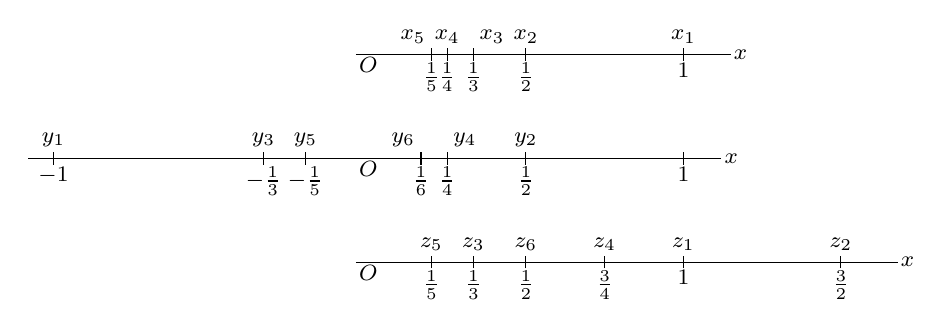
\begin{tikzpicture}[x=4cm,y=1.32cm,
      every node/.style={font=\footnotesize,inner sep=1pt}]
    % x_n
    \draw[line width=.45pt] (-.04,2) -- (1.15,2);
    \node[below] at (0,2) {\(O\)};
    \node[right] at (1.15,2) {\(x\)};
    \foreach \v in {.2,.25,.3333,.5,1}
      \draw[line width=.4pt] (\v,1.94) -- (\v,2.06);
    \node[above left=1pt] at (.2,2.05) {\(x_5\)};
    \node[above=1pt] at (.25,2.05) {\(x_4\)};
    \node[above right=1pt] at (.3333,2.05) {\(x_3\)};
    \node[above=1pt] at (.5,2.05) {\(x_2\)};
    \node[above=1pt] at (1,2.05) {\(x_1\)};
    \node[below] at (.2,1.95) {\(\frac15\)};
    \node[below] at (.25,1.95) {\(\frac14\)};
    \node[below] at (.3333,1.95) {\(\frac13\)};
    \node[below] at (.5,1.95) {\(\frac12\)};
    \node[below] at (1,1.95) {\(1\)};

    % y_n
    \draw[line width=.45pt] (-1.08,1) -- (1.12,1);
    \node[below] at (0,1) {\(O\)};
    \node[right] at (1.12,1) {\(x\)};
    \foreach \v in {-1,-.3333,-.2,.1667,.25,.5,1}
      \draw[line width=.4pt] (\v,.94) -- (\v,1.06);
    \node[above=1pt] at (-1,1.05) {\(y_1\)};
    \node[above=1pt] at (-.3333,1.05) {\(y_3\)};
    \node[above=1pt] at (-.2,1.05) {\(y_5\)};
    \node[above left=1pt] at (.1667,1.05) {\(y_6\)};
    \node[above right=1pt] at (.25,1.05) {\(y_4\)};
    \node[above=1pt] at (.5,1.05) {\(y_2\)};
    \node[below] at (-1,.95) {\(-1\)};
    \node[below] at (-.3333,.95) {\(-\frac13\)};
    \node[below] at (-.2,.95) {\(-\frac15\)};
    \node[below] at (.1667,.95) {\(\frac16\)};
    \node[below] at (.25,.95) {\(\frac14\)};
    \node[below] at (.5,.95) {\(\frac12\)};
    \node[below] at (1,.95) {\(1\)};

    % z_n
    \draw[line width=.45pt] (-.04,0) -- (1.68,0);
    \node[below] at (0,0) {\(O\)};
    \node[right] at (1.68,0) {\(x\)};
    \foreach \v in {.2,.3333,.5,.75,1,1.5}
      \draw[line width=.4pt] (\v,-.06) -- (\v,.06);
    \node[above=1pt] at (.2,.05) {\(z_5\)};
    \node[above=1pt] at (.3333,.05) {\(z_3\)};
    \node[above=1pt] at (.5,.05) {\(z_6\)};
    \node[above=1pt] at (.75,.05) {\(z_4\)};
    \node[above=1pt] at (1,.05) {\(z_1\)};
    \node[above=1pt] at (1.5,.05) {\(z_2\)};
    \node[below] at (.2,-.05) {\(\frac15\)};
    \node[below] at (.3333,-.05) {\(\frac13\)};
    \node[below] at (.5,-.05) {\(\frac12\)};
    \node[below] at (.75,-.05) {\(\frac34\)};
    \node[below] at (1,-.05) {\(1\)};
    \node[below] at (1.5,-.05) {\(\frac32\)};
  \end{tikzpicture}
  \caption{}
  \label{fig:3-1}
\end{figure}

\begin{mydef*}{}
我们称实数序列 \(\langle x_n\rangle\) \textbf{发散}，如果 \(\langle x_n\rangle\) 不收敛。
\end{mydef*}

由序列收敛的定义可知：
\[
\begin{aligned}
\langle x_n\rangle\text{ 发散}
&\iff(\forall\,a\in\R)\quad \lim_{n\to+\infty}x_n\neq a\\
&\iff(\forall\,a\in\R)(\exists\,\varepsilon_a>0)(\forall\,n\in\N)
   (\exists\,k_n\in\N,\ k_n\geqslant n)\\
&\hspace{7em}\Longrightarrow |x_{k_n}-a|\geqslant\varepsilon_a.
\end{aligned}
\]

\begin{sourceexample}{3}
证明：实数序列 \(\langle1+(-1)^n\rangle\) 发散。

事实上，\(\forall\,a\in\R\)，由
\[
\begin{aligned}
2=|2-a+a|
&\leqslant |2-a|+|a|\\
&=|1+(-1)^{2n}-a|+|1+(-1)^{2n-1}-a|
\end{aligned}
\]
推知
\[
|1+(-1)^{2n}-a|\geqslant1
\quad\text{或}\quad
|1+(-1)^{2n-1}-a|\geqslant1.
\]
因此
\[
\begin{aligned}
(\forall\,a\in\R)(\exists\,\varepsilon_a=1>0)(\forall\,n\in\N)
(\exists\,k_n\in\{2n,2n-1\},\ k_n\geqslant n)\\
\Longrightarrow |1+(-1)^{k_n}-a|\geqslant1.
\end{aligned}
\]
此即表明 \(\langle1+(-1)^n\rangle\) 发散。
\end{sourceexample}

直接从序列极限的定义可推出下述等价命题成立：
\[
\lim_{n\to+\infty}x_n=a
\iff
(\forall\,\varepsilon>0)(\exists\,N\in\N)
(\forall\,n\in\N,\ n\geqslant N)
\Longrightarrow |x_n-a|\leqslant M\varepsilon,
\]
这里 \(M\) 是与 \(n\) 无关的正数。

熟悉这一点，将给我们今后证明序列的极限带来方便。

现在我们介绍几个常用的方法。

\subsection{\texorpdfstring{用 \(\varepsilon\)-\(N\) 极限语言证明序列极限的方法}{用 ε-N 极限语言证明序列极限的方法}}

直接用 \(\varepsilon\)-\(N\) 极限语言证明 \(\lim_{n\to+\infty}x_n=a\) 没有万能的方法。总的原则是将差式
\(|x_n-a|\) 适当地放大成 \(|x_n-a|\leqslant A_n\) 的形式，使得表达式 \(A_n\) 的形式尽可能简洁，并由
\(A_n<\varepsilon\) 可方便地求出极限定义中所指的自然数 \(N\)。

下面就是几个一般的证明方法。

\subsubsection*{\texorpdfstring{1）直接变形求 \(A_n\)}{1）直接变形求 An}}

\begin{sourceexample}{4}
证明：
\[
\lim_{n\to+\infty}\sqrt[3]{n}\bigl(\sqrt[3]{n}-\sqrt[3]{n-1}\bigr)=0.
\]

\(\forall\,n\in\N\)，由于
\[
\begin{aligned}
&\left|\sqrt[3]{n}\bigl(\sqrt[3]{n}-\sqrt[3]{n-1}\bigr)-0\right|\\
&=\sqrt[3]{n}\bigl(\sqrt[3]{n}-\sqrt[3]{n-1}\bigr)\\
&=\frac{\sqrt[3]{n}\bigl(\sqrt[3]{n}-\sqrt[3]{n-1}\bigr)
\bigl(\sqrt[3]{n^2}+\sqrt[3]{n(n-1)}+\sqrt[3]{(n-1)^2}\bigr)}
{\sqrt[3]{n^2}+\sqrt[3]{n(n-1)}+\sqrt[3]{(n-1)^2}}\\
&=\frac{\sqrt[3]{n}}
{\sqrt[3]{n^2}+\sqrt[3]{n(n-1)}+\sqrt[3]{(n-1)^2}}
<\frac1{\sqrt[3]{n}}.
\end{aligned}
\]
故 \(\forall\,\varepsilon>0\)，由 \(\dfrac1{\sqrt[3]{n}}<\varepsilon\) 得到
\(n>\dfrac1{\varepsilon^3}\)。令
\[
N=\left[\frac1{\varepsilon^3}\right]+1,
\]
则
\[
\forall\,n\in\N,\quad n\geqslant N
\Longrightarrow
\left|\sqrt[3]{n}\bigl(\sqrt[3]{n}-\sqrt[3]{n-1}\bigr)-0\right|
<\frac1{\sqrt[3]{n}}<\varepsilon.
\]
因此
\[
\lim_{n\to+\infty}\sqrt[3]{n}\bigl(\sqrt[3]{n}-\sqrt[3]{n-1}\bigr)=0.
\]
\end{sourceexample}

\begin{sourceexample}{5}
证明：
\[
\lim_{n\to+\infty}
\left(\frac1{1\cdot2}+\frac1{2\cdot3}+\cdots+\frac1{n(n+1)}\right)=1.
\]

\(\forall\,n\in\N\)，由于
\[
\begin{aligned}
\frac1{1\cdot2}+\frac1{2\cdot3}+\cdots+\frac1{n(n+1)}
&=\left(1-\frac12\right)+\left(\frac12-\frac13\right)
 +\cdots+\left(\frac1n-\frac1{n+1}\right)\\
&=1-\frac1{n+1},
\end{aligned}
\]
故
\[
\left|
\frac1{1\cdot2}+\frac1{2\cdot3}+\cdots+\frac1{n(n+1)}-1
\right|
=\frac1{n+1}<\frac1n.
\]
\(\forall\,\varepsilon>0\)，由 \(\dfrac1n<\varepsilon\) 得到
\(n>\dfrac1\varepsilon\)。令
\[
N=\left[\frac1\varepsilon\right]+1,
\]
则
\[
\forall\,n\in\N,\quad n\geqslant N
\Longrightarrow
\left|
\frac1{1\cdot2}+\frac1{2\cdot3}+\cdots+\frac1{n(n+1)}-1
\right|<\varepsilon.
\]
因此
\[
\lim_{n\to+\infty}
\left(\frac1{1\cdot2}+\frac1{2\cdot3}+\cdots+\frac1{n(n+1)}\right)=1.
\]
\end{sourceexample}

\subsubsection*{\texorpdfstring{2）利用不等式求 \(A_n\)}{2）利用不等式求 An}}

\begin{sourceexample}{6}
证明：
\[
\lim_{n\to+\infty}
\frac{1\cdot3\cdots(2n-1)}{2\cdot4\cdots2n}=0.
\]

由不等式
\[
\frac{a+b}{2}\geqslant\sqrt{ab}\qquad(a\geqslant0,\ b\geqslant0)
\]
得到
\[
2=\frac{1+3}{2}\geqslant\sqrt{1\cdot3},\qquad
4=\frac{3+5}{2}\geqslant\sqrt{3\cdot5},\qquad\ldots,
\]
\[
2n=\frac{(2n-1)+(2n+1)}2\geqslant\sqrt{(2n-1)(2n+1)}.
\]
将这些不等式相乘得
\[
\begin{aligned}
2\cdot4\cdots2n
&\geqslant
\sqrt{1\cdot3}\sqrt{3\cdot5}\cdots\sqrt{(2n-1)(2n+1)}\\
&=1\cdot3\cdots(2n-1)\sqrt{2n+1}.
\end{aligned}
\]
由此得到
\[
\frac{1\cdot3\cdots(2n-1)}{2\cdot4\cdots2n}
<\frac1{\sqrt{2n+1}}<\frac1{\sqrt n}.
\]
\(\forall\,\varepsilon>0\)，由 \(\dfrac1{\sqrt n}<\varepsilon\) 得到
\(n>\dfrac1{\varepsilon^2}\)。令
\[
N=\left[\frac1{\varepsilon^2}\right]+1,
\]
则
\[
\forall\,n\in\N,\quad n\geqslant N
\Longrightarrow
\left|
\frac{1\cdot3\cdots(2n-1)}{2\cdot4\cdots2n}-0
\right|
<\frac1{\sqrt n}<\varepsilon.
\]
因此
\[
\lim_{n\to+\infty}
\frac{1\cdot3\cdots(2n-1)}{2\cdot4\cdots2n}=0.
\]
\end{sourceexample}

\begin{sourceexample}{7}
证明：
\[
\lim_{n\to+\infty}\frac1{\sqrt[n]{n!}}=0.
\]

由于 \(\forall\,n\in\N\)，
\[
\begin{aligned}
(n!)^2=n!\cdot n!
&=1\cdot n\cdot2\cdot(n-1)\cdots k(n-k+1)\cdots n\cdot1,
\end{aligned}
\]
并且
\[
\forall\,k,n\in\N,\quad k\leqslant n
\Longrightarrow k(n-k+1)\geqslant n,
\]
故
\[
(n!)^2\geqslant n\cdot n\cdots n=n^n.
\]
由此推得
\[
\sqrt[n]{n!}\geqslant\sqrt n,
\qquad\text{或}\qquad
\frac1{\sqrt[n]{n!}}\leqslant\frac1{\sqrt n}.
\]
\(\forall\,\varepsilon>0\)，由 \(\dfrac1{\sqrt n}<\varepsilon\) 得到
\(n>\dfrac1{\varepsilon^2}\)。令
\[
N=\left[\frac1{\varepsilon^2}\right]+1,
\]
则
\[
\forall\,n\in\N,\quad n\geqslant N
\Longrightarrow
\left|\frac1{\sqrt[n]{n!}}-0\right|
\leqslant\frac1{\sqrt n}<\varepsilon.
\]
因此
\[
\lim_{n\to+\infty}\frac1{\sqrt[n]{n!}}=0.
\]
\end{sourceexample}

\subsubsection*{\texorpdfstring{3）利用二项式展开求 \(A_n\)}{3）利用二项式展开求 An}}

\begin{sourceexample}{8}
证明：\(\forall\,q\in\R,\ |q|<1\)，
\[
\lim_{n\to+\infty}q^n=0.
\]

若 \(q=0\)，则结论显然成立。

若 \(q\neq0\)，则由于 \(|q|<1\)，有 \(\dfrac1{|q|}>1\)。令
\[
a=\frac1{|q|}-1,
\]
则 \(a>0\)，并且
\[
|q|=\frac1{1+a},\qquad |q|^n=\frac1{(1+a)^n}.
\]
由二项式展开公式得到
\[
(1+a)^n=1+na+\frac{n(n-1)}2a^2+\cdots+a^n>na,
\]
所以
\[
|q^n-0|=|q|^n=\frac1{(1+a)^n}<\frac1{na}.
\]
\(\forall\,\varepsilon>0\)，由 \(\dfrac1{na}<\varepsilon\) 得到
\(n>\dfrac1{a\varepsilon}\)。令
\[
N=\left[\frac1{a\varepsilon}\right]+1,
\]
则
\[
\forall\,n\in\N,\quad n\geqslant N
\Longrightarrow |q^n-0|<\frac1{na}<\varepsilon.
\]
因此
\[
\lim_{n\to+\infty}q^n=0.
\]
\end{sourceexample}

\begin{sourceexample}{9}
证明：\(\forall\,q\in\R,\ |q|<1\)，
\[
\lim_{n\to+\infty}nq^n=0.
\]

若 \(q=0\)，则结论显然成立。

若 \(q\neq0\)，则像上一题一样，令
\[
a=\frac1{|q|}-1>0.
\]
于是
\[
n|q|^n=\frac{n}{(1+a)^n}\qquad(n\in\N).
\]
由于
\[
(1+a)^n
=1+na+\frac{n(n-1)}2a^2+\cdots+a^n
>\frac{n(n-1)}2a^2,
\]
故
\[
|nq^n-0|
=n|q|^n
<\frac{n}{\frac{n(n-1)}2a^2}
=\frac2{(n-1)a^2}
\qquad(n\geqslant2).
\]
\(\forall\,\varepsilon>0\)，由
\(\dfrac2{(n-1)a^2}<\varepsilon\) 得到
\(n>1+\dfrac2{a^2\varepsilon}\)。令
\[
N=1+\left[1+\frac2{a^2\varepsilon}\right],
\]
则
\[
\forall\,n\in\N,\quad n\geqslant N
\Longrightarrow
|nq^n-0|<\frac2{(n-1)a^2}<\varepsilon.
\]
因此
\[
\lim_{n\to+\infty}nq^n=0.
\]
\end{sourceexample}

\subsubsection*{\texorpdfstring{4）分析法求 \(A_n\)}{4）分析法求 An}}

\begin{sourceexample}{10}
证明：
\[
\lim_{n\to+\infty}\frac{a^n}{n!}=0
\qquad(a\neq0).
\]

首先，\(\forall\,n,m\in\N\) 且 \(m\leqslant n\)，我们有
\[
\begin{aligned}
\left|\frac{a^n}{n!}-0\right|
&=\frac{|a|^n}{n!}\\
&=\left(\frac{|a|}{1}\frac{|a|}{2}\cdots\frac{|a|}{m-1}\right)
  \left(\frac{|a|}{m}\cdots\frac{|a|}{n-1}\right)\frac{|a|}{n}.
\end{aligned}
\]
若取 \(m\geqslant|a|\)，则
\[
\left|\frac{a^n}{n!}-0\right|
<\frac{|a|^{m-1}}{(m-1)!}\cdot1\cdots1\cdot\frac{|a|}{n}
=\frac Mn,
\]
这里
\[
M=\frac{|a|^m}{(m-1)!}>0.
\]
\(\forall\,\varepsilon>0\)，由 \(\dfrac Mn<\varepsilon\) 得到
\(n>\dfrac M\varepsilon\)。令
\[
N=\max\left(m,\left[\frac M\varepsilon\right]+1\right),
\]
则
\[
\forall\,n\in\N,\quad n\geqslant N
\Longrightarrow
\left|\frac{a^n}{n!}-0\right|<\frac Mn<\varepsilon.
\]
因此
\[
\lim_{n\to+\infty}\frac{a^n}{n!}=0.
\]
\end{sourceexample}

\begin{sourceexample}{11}
证明：若
\[
\lim_{n\to+\infty}x_n=a,
\]
则
\[
\lim_{n\to+\infty}\frac{x_1+x_2+\cdots+x_n}{n}=a.
\]

由于 \(\lim_{n\to+\infty}x_n=a\)，故由定义
\[
(\forall\,\varepsilon>0)(\exists\,N_1\in\N)
(\forall\,n\in\N,\ n\geqslant N_1)
\Longrightarrow |x_n-a|<\frac\varepsilon2.
\]
因此 \(\forall\,n\geqslant N_1\)，
\[
\begin{aligned}
\left|\frac{x_1+x_2+\cdots+x_n}{n}-a\right|
&=\left|\frac{x_1+x_2+\cdots+x_n-na}{n}\right|\\
&\leqslant
\left|\frac{(x_1-a)+\cdots+(x_{N_1}-a)}{n}\right|\\
&\quad+
\left|\frac{(x_{N_1+1}-a)+\cdots+(x_n-a)}{n}\right|\\
&<\frac{|(x_1-a)+\cdots+(x_{N_1}-a)|}{n}
+\frac{n-N_1}{n}\frac\varepsilon2\\
&<\frac Mn+\frac\varepsilon2,
\end{aligned}
\]
这里
\[
M=|(x_1-a)+\cdots+(x_{N_1}-a)|\geqslant0.
\]
由 \(\dfrac Mn<\dfrac\varepsilon2\) 得到
\(n>\dfrac{2M}{\varepsilon}\)。令
\[
N=\max\left(N_1,\left[\frac{2M}{\varepsilon}\right]+1\right),
\]
则
\[
\begin{aligned}
\forall\,n\in\N,\quad n\geqslant N
&\Longrightarrow
\left|\frac{x_1+x_2+\cdots+x_n}{n}-a\right|
<\frac Mn+\frac\varepsilon2\\
&<\frac\varepsilon2+\frac\varepsilon2=\varepsilon.
\end{aligned}
\]
因此
\[
\lim_{n\to+\infty}\frac{x_1+x_2+\cdots+x_n}{n}=a.
\]
\end{sourceexample}

\subsection*{习 题}
\begin{exercise}
  \item 证明下列结论等价：
  \begin{enumerate}[label=\arabic*)]
    \item \(\displaystyle\lim_{n\to+\infty}x_n=a\)；
    \item \((\forall\,\varepsilon>0)(\exists\,N\in\N)
      (\forall\,n\in\N,\ n\geqslant N)
      \Longrightarrow |x_n-a|<M\varepsilon\)，其中 \(M\) 为常数；
    \item \((\forall\,k\in\N)(\exists\,N\in\N)
      (\forall\,n\in\N,\ n\geqslant N)
      \Longrightarrow |x_n-a|<\dfrac1k\)。
  \end{enumerate}
\end{exercise}

\begin{exercise}
  \item 证明：实数序列 \(\langle(-1)^n\rangle\) 发散。
\end{exercise}

\begin{exercise}
  \item 证明：\(\forall\,a\in\R\)，
  \[
  \lim_{n\to+\infty}\frac{[na]}n=a.
  \]
\end{exercise}

\begin{exercise}
  \item 证明：若 \(\displaystyle\lim_{n\to+\infty}x_n=a\)，则
  \[
  \lim_{n\to+\infty}|x_n|=|a|.
  \]
  举例说明逆命题不成立。
\end{exercise}

\begin{exercise}
  \item 证明：
  \[
  \lim_{n\to+\infty}x_n=a
  \]
  当且仅当
  \[
  \lim_{n\to+\infty}x_{2n}
  =\lim_{n\to+\infty}x_{2n+1}=a.
  \]
\end{exercise}

\begin{exercise}
  \item 用 \(\varepsilon\)-\(N\) 语言证明下列各极限：
  \begin{enumerate}[label=\arabic*)]
    \item \(\displaystyle\lim_{n\to+\infty}\frac{n!}{n^n}=0\)；
    \item \(\displaystyle\lim_{n\to+\infty}\sqrt[n]{a}=1\quad(a>0)\)；
    \item \(\displaystyle\lim_{n\to+\infty}\frac{n^k}{a^n}=0
      \quad(a>1,\ k\in\N)\)；
    \item \(\displaystyle\lim_{n\to+\infty}\sqrt[n]{n^k}=1
      \quad(k\in\N)\)；
    \item \(\displaystyle\lim_{n\to+\infty}\left(\sqrt[k]{n}\right)^{1/n}=1
      \quad(k\in\N)\)；
    \item \(\displaystyle\lim_{n\to+\infty}
      \left(\frac1{n^2}+\frac1{(n+1)^2}+\cdots+\frac1{(2n)^2}\right)=0\)；
    \item \(\displaystyle\lim_{n\to+\infty}
      \left(\frac1{n^2}+\frac2{n^2}+\cdots+\frac n{n^2}\right)=\frac12\)；
    \item \(\displaystyle\lim_{n\to+\infty}
      \left(\frac12+\frac2{2^2}+\cdots+\frac n{2^n}\right)=2\)；
    \item \(\displaystyle\lim_{n\to+\infty}
      \frac32\cdot\frac54\cdots
      \frac{2^{2^n}+1}{2^{2^n}}=2\)；
    \item \(\displaystyle\lim_{n\to+\infty}
      \left(\frac12+\frac3{2^2}+\cdots+\frac{2n-1}{2^n}\right)=3\)。
  \end{enumerate}
\end{exercise}

\begin{exercise}
  \item 设 \(\langle x_n\rangle\) 是任一实数序列，使得
  \[
  \lim_{n\to+\infty}(x_{n+1}-x_n)=0.
  \]
  证明：
  \[
  \lim_{n\to+\infty}\frac{x_n}{n}=0.
  \]
\end{exercise}

\begin{exercise}
  \item 设 \(a_0,a_1,\ldots,a_k\in\R\)，使得
  \[
  a_0+a_1+\cdots+a_k=0.
  \]
  证明：
  \[
  \lim_{n\to+\infty}
  \left(a_0\sqrt n+a_1\sqrt{n+1}+\cdots+a_k\sqrt{n+k}\right)=0.
  \]
\end{exercise}

\begin{exercise}
  \item 设 \(\langle x_n\rangle\) 是任一实数序列，并且
  \[
  \lim_{n\to+\infty}x_n=a.
  \]
  \begin{enumerate}[label=\arabic*)]
    \item 证明：
    \[
    \lim_{n\to+\infty}\frac{x_1+2x_2+\cdots+nx_n}{n^2}=\frac a2.
    \]
    \item 利用 1）的结论计算下列各极限值（\(0<a<1\)）：
    \[
    \lim_{n\to+\infty}
    \frac1{n^2}\left(a+2^2a^2+\cdots+n^2a^n\right),
    \]
    \[
    \lim_{n\to+\infty}
    \frac1{n^2}\left(1+\sqrt{2^3}+\sqrt[3]{3^4}
    +\cdots+\sqrt[n]{n^{n+1}}\right).
    \]
  \end{enumerate}
\end{exercise}

\begin{exercise}
  \item 分别利用极限定义及反证法证明序列 \(\langle\sin n\rangle\) 发散。
\end{exercise}

\begin{exercise}
  \item 设 \(\langle a_n\rangle\) 是一实数序列，令
  \[
  b_n=a_{n-1}+2a_n\qquad(n\in\N,\ n\geqslant2).
  \]
  证明：若序列 \(\langle b_n\rangle\) 收敛，则序列 \(\langle a_n\rangle\) 也收敛，并且
  \[
  \lim_{n\to+\infty}b_n=3\lim_{n\to+\infty}a_n.
  \]
\end{exercise}

\begin{exercise}
  \item 设实数序列 \(\langle a_n\rangle\) 满足条件
  \[
  \lim_{n\to+\infty}(a_n-a_{n-2})=0.
  \]
  证明：
  \[
  \lim_{n\to+\infty}\frac1n(a_n-a_{n-1})=0.
  \]
\end{exercise}

\begin{exercise}
  \item 设 \(X\subset\R\) 是任一非空集合。证明：\(X\) 是闭集的充分必要条件是
  \[
  \forall\,x_n\in X\ (n\in\N),\quad
  x_n\to x\ (n\to+\infty)
  \Longrightarrow x\in X.
  \]
\end{exercise}

\section{收敛序列的性质}

\subsection{收敛序列的一般性质}

\begin{myproperty}{}{limit-uniqueness}
如果实数序列 \(\langle x_n\rangle\) 收敛，则此序列的极限是唯一的。
\end{myproperty}

\begin{proof}
设 \(\lim_{n\to+\infty}x_n=a\)，\(\lim_{n\to+\infty}x_n=b\)，并且 \(a\ne b\)。于是由 \(\R\) 的 Hausdorff 分离性，存在 \(\delta>0\) 使得
\[
B(a,\delta)\cap B(b,\delta)=\varnothing.
\]
另一方面，对 \(\delta>0\)，存在 \(N_1,N_2\in\N\)，使得
\[
\forall n\in\N,\quad n\geqslant N_1\Longrightarrow x_n\in B(a,\delta),
\]
\[
\forall n\in\N,\quad n\geqslant N_2\Longrightarrow x_n\in B(b,\delta).
\]
令 \(N=\max(N_1,N_2)\)，则
\[
\forall n\in\N,\quad n\geqslant N
\Longrightarrow x_n\in B(a,\delta)\cap B(b,\delta).
\]
这与 \(B(a,\delta)\cap B(b,\delta)=\varnothing\) 相矛盾。因此 \(a=b\)。
\end{proof}

\begin{myproperty}{}{finite-modification-preserves-limit}
如果 \(\lim_{n\to+\infty}x_n=a\)，则任意改变 \(\langle x_n\rangle\) 的有限多项后所得新的实数序列 \(\langle y_n\rangle\) 也有
\[
\lim_{n\to+\infty}y_n=a.
\]
\end{myproperty}

证明留给读者。

\begin{myproperty}{}{convergent-sequence-bounded}
如果实数序列 \(\langle x_n\rangle\) 收敛，则 \(\langle x_n\rangle\) 是有界的，即
\[
(\exists M>0)(\forall n\in\N)\Longrightarrow |x_n|\leqslant M.
\]
\end{myproperty}

\begin{proof}
设 \(\lim_{n\to+\infty}x_n=a\)。于是对 \(\varepsilon=1\)，存在 \(N\in\N\)，使得
\[
\forall n\in\N,\quad n\geqslant N\Longrightarrow |x_n-a|<1
\Longrightarrow |x_n|\leqslant |x_n-a|+|a|<1+|a|.
\]
令
\[
M=\max(|x_1|,|x_2|,\dots,|x_{N-1}|,1+|a|),
\]
则 \(\forall n\in\N\)，\(|x_n|\leqslant M\)。
\end{proof}

\begin{myproperty}{}{subsequence-preserves-limit}
如果 \(\lim_{n\to+\infty}x_n=a\)，则对任一映射 \(k\colon\N\to\N\)，若
\[
k(n)<k(n+1)\quad(\forall n\in\N),
\]
也有 \(\lim_{n\to+\infty}x_{k(n)}=a\)。
\end{myproperty}

序列 \(\langle x_{k(n)}\rangle\) 称为 \(\langle x_n\rangle\) 的子序列，\(\langle x_{k(n)}\rangle\) 也常记为 \(\langle x_{k_n}\rangle\)。

\begin{proof}
因为 \(\lim_{n\to+\infty}x_n=a\)，所以由定义
\[
(\forall\varepsilon>0)(\exists N\in\N)(\forall n\in\N, n\geqslant N)
\Longrightarrow |x_n-a|<\varepsilon.
\]
现设 \(k\colon\N\to\N\) 是任一严格单调上升映射。由归纳法可证
\[
\forall n\in\N,\quad k(n)\geqslant n.
\]
由此推得
\[
\forall n\in\N,\quad n\geqslant N\Longrightarrow k(n)\geqslant N
\Longrightarrow |x_{k(n)}-a|<\varepsilon.
\]
因此 \(\lim_{n\to+\infty}x_{k(n)}=a\)。
\end{proof}

\begin{sourceexample}{1}
利用\rprop{property:subsequence-preserves-limit}证明实数序列 \(\langle1+(-1)^n\rangle\) 发散。

定义严格单调上升映射 \(k,l\colon\N\to\N\) 如下：
\[
k(n)=2n,\quad l(n)=2n-1\quad(\forall n\in\N).
\]
那么
\[
1+(-1)^{k(n)}=2,\quad 1+(-1)^{l(n)}=0\quad(\forall n\in\N).
\]
因此
\[
\lim_{n\to+\infty}[1+(-1)^{k(n)}]=2,\quad
\lim_{n\to+\infty}[1+(-1)^{l(n)}]=0.
\]
由\rprop{property:subsequence-preserves-limit}知，序列 \(\langle1+(-1)^n\rangle\) 发散。
\end{sourceexample}

\begin{sourceexample}{2}
设 \(p\in\N\)，\(\langle x_n\rangle\) 是一实数序列，满足
\[
x_n=x_{n+p}\quad(\forall n\in\N).
\]
证明：若 \(\lim_{n\to+\infty}x_n=a\)，则 \(x_n=a\ (\forall n\in\N)\)。

为此，考虑 \(p\) 个严格单调上升映射 \(k^{(i)}\colon\N\to\N\ (i=1,2,\dots,p)\)，它们定义为
\[
k^{(i)}(n)=i+(n-1)p,\quad \forall n\in\N\quad(i=1,2,\dots,p).
\]
由于 \(\lim_{n\to+\infty}x_n=a\)，故
\[
\forall i=1,2,\dots,p,\quad
\lim_{n\to+\infty}x_{k^{(i)}(n)}=a.
\]
另一方面，由假设 \(x_n=x_{n+p}\ (\forall n\in\N)\)，我们有
\[
x_{k^{(i)}(n)}=x_{k^{(i)}(n+1)},\quad
\forall n\in\N\quad(i=1,2,\dots,p).
\]
因此 \(x_{k^{(i)}(n)}\equiv a\ (\forall n\in\N)\ (i=1,2,\dots,p)\)，从而 \(x_n\equiv a\ (\forall n\in\N)\)。
\end{sourceexample}

\subsection{收敛序列极限的运算性质}

\begin{myproperty}{}{limit-arithmetic}
设 \(\lim_{n\to+\infty}x_n=a\)，\(\lim_{n\to+\infty}y_n=b\)。则实数序列
\[
\langle x_n+y_n\rangle,\quad \langle x_ny_n\rangle,\quad
\left\langle\frac{x_n}{y_n}\right\rangle\quad(b\ne0)
\]
也收敛，并且
\begin{enumerate}[label=\arabic*)]
  \item \(\displaystyle\lim_{n\to+\infty}(x_n+y_n)=a+b\)；
  \item \(\displaystyle\lim_{n\to+\infty}x_ny_n=ab\)；
  \item \(\displaystyle\lim_{n\to+\infty}\frac{x_n}{y_n}=\frac ab\quad(b\ne0)\)。
\end{enumerate}
\end{myproperty}

\begin{proof}

因为 \(\lim_{n\to+\infty}x_n=a\)，\(\lim_{n\to+\infty}y_n=b\)，所以
\[
(\forall\varepsilon>0)(\exists N\in\N)(\forall n\in\N, n\geqslant N)
\Longrightarrow
\begin{cases}
|x_n-a|<\varepsilon,\\
|y_n-b|<\varepsilon,\quad |y_n|<|b|+\varepsilon.
\end{cases}
\]

由此推得

\[\forall n \in \mathbb{N}, n \geqslant N\]

\[\Longrightarrow
\begin{cases}
|(x_n+y_n)-(a+b)|\leqslant|x_n-a|+|y_n-b|<2\varepsilon,\\
|x_ny_n-ab|\leqslant|y_n||x_n-a|+|a||y_n-b|
<( |a|+|b|+\varepsilon)\varepsilon.
\end{cases}
\]

因此\(\langle x_n + y_n \rangle\) 及\(\langle x_n y_n \rangle\) 收敛,并且\(\lim_{n \to +\infty} (x_n + y_n) = a + b\) ,\(\lim_{n \to +\infty} x_n y_n = ab\) .

若 \(b\ne0\)，则不妨设 \(0<\varepsilon<|b|/2\)。由 \(|y_n-b|<\varepsilon\) 推得
\[
|y_n|>|b|-\varepsilon\geqslant\frac{|b|}{2}\quad(\forall n\in\N,\ n\geqslant N).
\]
因此
\[
\begin{aligned}
\forall n\in\N,\quad n\geqslant N\Longrightarrow
\left|\frac{x_n}{y_n}-\frac ab\right|
&=\frac{|x_nb-y_na|}{|b|\,|y_n|}\\
&\leqslant\frac{2}{|b|^2}\bigl(|x_nb-ab|+|y_na-ab|\bigr)\\
&\leqslant\frac{2(|a|+|b|)}{|b|^2}\varepsilon.
\end{aligned}
\]

从而 \(\left\langle x_n/y_n\right\rangle\) 收敛，并且
\(\lim_{n\to+\infty}x_n/y_n=a/b\)。

\end{proof}

\begin{mycor*}{}
若 \(\lim_{n\to+\infty}x_n=a\)，\(b\in\R\)，则
\[
\lim_{n\to+\infty}(x_n+b)=a+b,\qquad
\lim_{n\to+\infty}x_nb=ab,
\]
\[
\lim_{n\to+\infty}\frac1{x_n}=\frac1a\quad(a\ne0).
\]
\end{mycor*}

\begin{sourceexample}{3}
由于 \(\forall p\in\N\)，\(\lim_{n\to+\infty}1/n^p=0\)，及
\[
\begin{aligned}
&\frac{a_k n^k+a_{k-1}n^{k-1}+\cdots+a_1n+a_0}
       {b_m n^m+b_{m-1}n^{m-1}+\cdots+b_1n+b_0}\\
&\qquad=
\frac{a_k+a_{k-1}/n+\cdots+a_1/n^{k-1}+a_0/n^k}
     {b_m+b_{m-1}/n+\cdots+b_1/n^{m-1}+b_0/n^m}\,n^{k-m}.
\end{aligned}
\]

因此

\[\lim_{n \to +\infty} \frac{a_k n^k + a_{k-1} n^{k-1} + \cdots + a_1 n + a_0}{b_m n^m + b_{m-1} n^{m-1} + \cdots + b_1 n + b_0}\]

\[= \begin{cases} \dfrac{a_k}{b_m}, & k=m, \\ 0, & k<m. \end{cases}\]

从而

\[\lim_{n\to+\infty} \frac{3n^3-1}{2n^3+n^2+1} = \frac{3}{2},\]

\[\lim_{n\to+\infty} \frac{4n^2+n+1}{5n^3+2n-1} = 0.\]
\end{sourceexample}

\subsection{收敛序列的不等式性质}

\begin{myproperty}{}{limit-eventual-order}
如果 \(\lim_{n\to+\infty}x_n=a\)，并且 \(a>r\)（\(a<r\)），则
\[
(\exists N\in\N)(\forall n\in\N, n\geqslant N)
\Longrightarrow x_n>r\quad(x_n<r).
\]
\end{myproperty}

\begin{proof}
设 \(a>r\)。对于 \(\varepsilon=a-r>0\)，存在 \(N\in\N\)，使得
\[
\forall n\in\N,\quad n\geqslant N\Longrightarrow |x_n-a|<a-r
\Longrightarrow x_n>a-(a-r)=r.
\]
类似可证 \(a<r\) 的情形。
\end{proof}

\begin{myproperty}{}{limit-strict-comparison}
如果 \(\lim_{n\to+\infty}x_n=a\)，\(\lim_{n\to+\infty}y_n=b\)，并且 \(a>b\)（\(a<b\)），则
\[
(\exists N\in\N)(\forall n\in\N, n\geqslant N)
\Longrightarrow x_n>y_n\quad(x_n<y_n).
\]
\end{myproperty}

\begin{proof}
设 \(a>b\)。于是存在 \(r\in\R\)，使得 \(a>r>b\)。由
\[
\lim_{n\to+\infty}x_n=a>r>b=\lim_{n\to+\infty}y_n
\]
及\rprop{property:limit-eventual-order}知，存在 \(N_1,N_2\in\N\)，使得
\[
\forall n\in\N,\quad n\geqslant N_1\Longrightarrow x_n>r,
\]
\[
\forall n\in\N,\quad n\geqslant N_2\Longrightarrow y_n<r.
\]
令 \(N=\max(N_1,N_2)\)，则
\[
\forall n\in\N,\quad n\geqslant N\Longrightarrow x_n>y_n.
\]
对 \(a<b\)，可类似证明。
\end{proof}

\begin{myproperty}{}{limit-preserves-order}
设 \(\lim_{n\to+\infty}x_n=a\)，\(\lim_{n\to+\infty}y_n=b\)，则
\[
\forall n\geqslant N,\quad x_n\geqslant y_n\quad(x_n\leqslant y_n)
\Longrightarrow a\geqslant b\ (a\leqslant b).
\]
\end{myproperty}

\begin{proof}
用反证法，由\rprop{property:limit-strict-comparison}立即推出。
\end{proof}

\begin{mycor*}{}
如果 \(\lim_{n\to+\infty}x_n=a\)，并且 \(\forall n\geqslant N\)，
\(x_n\geqslant r\ (x_n\leqslant r)\)，则 \(a\geqslant r\ (a\leqslant r)\)。
\end{mycor*}

注意，即使在\rprop{property:limit-preserves-order}中将不等号“\(\geqslant\)（\(\leqslant\)）”换成严格不等号“\(>\)（\(<\)）”，也不一定有 \(a>b\ (a<b)\)。例如，取
\[
x_n=\frac1n,\qquad y_n=-\frac1n\quad(n\in\N).
\]
显然有 \(x_n>y_n\ (\forall n\in\N)\)，但是
\(\lim_{n\to+\infty}x_n=\lim_{n\to+\infty}y_n=0\)。

\begin{myproperty}{}{squeeze-theorem}
设实数序列 \(\langle x_n\rangle\)、\(\langle y_n\rangle\)、\(\langle z_n\rangle\) 满足下述条件：
\begin{enumerate}[label=\arabic*)]
  \item \(x_n\leqslant z_n\leqslant y_n\quad(\forall n\in\N, n\geqslant N)\)；
  \item \(\displaystyle\lim_{n\to+\infty}x_n=\lim_{n\to+\infty}y_n=a\)，
\end{enumerate}
则 \(\lim_{n\to+\infty}z_n=a\)。
\end{myproperty}

\begin{proof}
由已知条件，对任意 \(\varepsilon>0\)，存在 \(N_0\in\N\)，\(N_0\geqslant N\)，使得
\[
\forall n\in\N,\quad n\geqslant N_0
\Longrightarrow |x_n-a|<\varepsilon,\quad |y_n-a|<\varepsilon.
\]
由此推得
\[
a-\varepsilon<x_n\leqslant z_n\leqslant y_n<a+\varepsilon
\Longrightarrow |z_n-a|<\varepsilon.
\]
因此 \(\lim_{n\to+\infty}z_n=a\)。
\end{proof}

\rprop{property:squeeze-theorem}常称为序列极限的两边夹法则。

\begin{sourceexample}{4}
设
\[
x_n=\frac{n}{\sqrt{n^2+n}},\qquad
y_n=\frac{n}{\sqrt{n^2+1}},
\]
\[
z_n=\frac1{\sqrt{n^2+1}}+\frac1{\sqrt{n^2+2}}+\cdots+\frac1{\sqrt{n^2+n}}
\quad(n\in\N).
\]
证明：
\[
\lim_{n\to+\infty}x_n=\lim_{n\to+\infty}y_n=\lim_{n\to+\infty}z_n=1.
\]
首先由不等式
\[
1<\sqrt{1+\frac1{n^2}}\leqslant\sqrt{1+\frac1n}<1+\frac1n
\quad(\forall n\in\N)
\]
及\rprop{property:squeeze-theorem}推得
\[
\lim_{n\to+\infty}\sqrt{1+\frac1n}
=\lim_{n\to+\infty}\sqrt{1+\frac1{n^2}}=1.
\]
因此
\[
\lim_{n\to+\infty}x_n=1,\qquad \lim_{n\to+\infty}y_n=1.
\]
另一方面，由于
\[
x_n=\underbrace{\frac1{\sqrt{n^2+n}}+\cdots+\frac1{\sqrt{n^2+n}}}_{n\text{ 项}}
<z_n<\frac{n}{\sqrt{n^2+1}}=y_n,
\]
故 \(x_n\leqslant z_n\leqslant y_n\ (\forall n\in\N)\)。从而由\rprop{property:squeeze-theorem}得到
\[
\lim_{n\to+\infty}z_n=1.
\]
\end{sourceexample}

\begin{sourceexample}{5}
设 \(\langle x_n\rangle\) 是任一实数序列，并且
\(x_n\leqslant x_{n+1}\ (\forall n\in\N)\)。证明：若
\[
\lim_{n\to+\infty}\frac{x_1+x_2+\cdots+x_n}{n}=a,
\]
则 \(\lim_{n\to+\infty}x_n=a\)。

令 \(y_n=(x_1+x_2+\cdots+x_n)/n\)。首先有
\[
y_n\leqslant x_n\quad(\forall n\in\N).
\]
现在任意固定 \(n\in\N\)。\(\forall m\geqslant n\)，
\[
y_m=\frac{x_1+\cdots+x_n}{m}+\frac{x_{n+1}+\cdots+x_m}{m}
\geqslant\frac{x_1+\cdots+x_n}{m}+\left(\frac{m-n}{m}\right)x_n.
\]
两边令 \(m\to+\infty\)，由\rprop{property:limit-preserves-order}得到
\[
a=\lim_{m\to+\infty}y_m
\geqslant\lim_{m\to+\infty}\frac{x_1+\cdots+x_n}{m}
+\lim_{m\to+\infty}\left(\frac{m-n}{m}\right)x_n=x_n.
\]
由此得到
\[
y_n\leqslant x_n\leqslant a\quad(\forall n\in\N).
\]
由于 \(\lim_{n\to+\infty}y_n=a\)，故由\rprop{property:squeeze-theorem}立即推得
\(\lim_{n\to+\infty}x_n=a\)。
\end{sourceexample}

\subsection*{习 题}

\begin{exercise}
  \item 设 \(\langle x_n\rangle\) 是任一实数序列，满足
  \(x_n\leqslant x_{n+1}\ (\forall n\in\N)\) 或
  \(x_n\geqslant x_{n+1}\ (\forall n\in\N)\)。如果存在
  \(\langle x_n\rangle\) 的一个子序列 \(\langle x_{k(n)}\rangle\)，使得
  \(\lim_{n\to+\infty}x_{k(n)}=a\)，则
  \(\lim_{n\to+\infty}x_n=a\)。
\end{exercise}

\begin{exercise}
  \item 计算下列各极限：
  \begin{enumerate}[label=\arabic*)]
    \item \(\displaystyle\lim_{n\to+\infty}\frac{\sqrt n}{\sqrt{n+\sqrt{n+\sqrt n}}}\)；
    \item \(\displaystyle\lim_{n\to+\infty}(\sqrt{n+1}-\sqrt n)\sqrt n\)；
    \item \(\displaystyle\lim_{n\to+\infty}\frac{\sqrt[3]{n^2+1}}{n+2}\)；
    \item \(\displaystyle\lim_{n\to+\infty}\left(\frac1{1\cdot3}+\frac1{2\cdot4}+\cdots+\frac1{n(n+2)}\right)\)；
    \item \(\displaystyle\lim_{n\to+\infty}\sum_{k=1}^{n}\frac1{(k+p)(k+p+q)}\quad(p,q\in\N)\)；
    \item \(\displaystyle\lim_{n\to+\infty}\sum_{k=1}^{n}\frac1{k(k+1)(k+2)}\)。
  \end{enumerate}
\end{exercise}

\begin{exercise}
  \item 设 \(\lim_{n\to+\infty}a_n=a\)，\(\lim_{n\to+\infty}b_n=b\)。证明：
  \begin{enumerate}[label=\arabic*)]
    \item \(\displaystyle\lim_{n\to+\infty}\max(a_n,b_n)=\max(a,b)\)；
    \item \(\displaystyle\lim_{n\to+\infty}\min(a_n,b_n)=\min(a,b)\)。
  \end{enumerate}
\end{exercise}

\begin{exercise}
  \item 设 \(\langle a_n\rangle\) 是任一严格正的实数序列，并且
  \(\lim_{n\to+\infty}a_n=0\)。证明：
  \begin{enumerate}[label=\arabic*)]
    \item 集合 \(\{n\in\N\mid \forall k\geqslant n, a_k\leqslant a_n\}\) 是无限集；
    \item 集合 \(\{n\in\N\mid \forall k\leqslant n, a_n\leqslant a_k\}\) 是无限集。
  \end{enumerate}
\end{exercise}

\begin{exercise}
  \item 设 \(\langle a_n\rangle\)、\(\langle b_n\rangle\) 是任意两个实数序列，并且
  \(\lim_{n\to+\infty}a_n=a\)，\(\lim_{n\to+\infty}b_n=b\)。定义序列 \(\langle c_n\rangle\) 如下：
  \[
  c_n=\frac1n(a_1b_n+a_2b_{n-1}+\cdots+a_nb_1)\quad(n\in\N).
  \]
  \begin{enumerate}[label=\arabic*)]
    \item 证明：存在常数 \(M>0\) 使得
    \[
    |c_n-ab|\leqslant\frac Mn\sum_{i=1}^{n}(|a_i-a|+|b_i-b|).
    \]
    \item 证明：\(\displaystyle\lim_{n\to+\infty}c_n=ab\)。
  \end{enumerate}
\end{exercise}

\begin{exercise}
  \item 设 \(\langle a_n\rangle\)、\(\langle b_n\rangle\) 是任意两个实数序列，满足：
  \begin{enumerate}[label=\arabic*)]
    \item \(\displaystyle\lim_{n\to+\infty}a_n=0\)，\(\displaystyle\lim_{n\to+\infty}b_n=0\)；
    \item 存在 \(M>0\) 使得 \(\forall n\in\N\)，
    \(|b_1|+|b_2|+\cdots+|b_n|\leqslant M\)。
  \end{enumerate}
  证明：
  \[
  \lim_{n\to+\infty}(a_1b_n+a_2b_{n-1}+\cdots+a_nb_1)=0.
  \]
\end{exercise}

\begin{exercise}
  \item 试利用两边夹法则证明下列各极限：
  \begin{enumerate}[label=\arabic*)]
    \item \(\displaystyle\lim_{n\to+\infty}\left[\frac1{(n+1)^2}+\frac1{(n+2)^2}+\cdots+\frac1{(2n)^2}\right]=0\)；
    \item \(\displaystyle\lim_{n\to+\infty}\sqrt[n]{a_1^n+a_2^n+\cdots+a_k^n}=\max_{1\leqslant i\leqslant k}a_i\quad(a_i\geqslant0, i=1,2,\dots,k)\)；
    \item \(\displaystyle\lim_{n\to+\infty}\sqrt[n]{\sqrt[n]{n}-1}=1\)；
    \item \(\displaystyle\lim_{n\to+\infty}\sqrt[n]{a_1a_2\cdots a_n}=a\)，这里 \(a_n>0\) 且 \(\displaystyle\lim_{n\to+\infty}a_n=a\)。
  \end{enumerate}
\end{exercise}

\begin{exercise}
  \item 设 \(\langle x_n\rangle\) 是任一实数序列。
  \begin{enumerate}[label=\arabic*)]
    \item 证明：如果子序列 \(\langle x_{2n}\rangle\)、\(\langle x_{2n+1}\rangle\)、\(\langle x_{3n}\rangle\) 收敛，那么序列 \(\langle x_n\rangle\) 收敛；
    \item 设 \(a,b\in\N\) 是两个互质自然数，\(u,v\in\N\) 使得 \(bv-au=1\)。假设子序列 \(\langle x_{bn}\rangle\) 收敛，并且 \(\forall r\in\{0,1,\dots,a-1\}\)，子序列 \(\langle x_{an+r}\rangle\) 收敛。证明：子序列 \(\langle x_{bn}\rangle\)、\(\langle x_{an+r}\rangle\) 及 \(\langle x_{abn+bvr}\rangle\) 收敛于同一极限 \(l\)，由此推出序列 \(\langle x_n\rangle\) 收敛于 \(l\)。
  \end{enumerate}
\end{exercise}

\begin{exercise}
  \item 设 \(\varphi\colon\N\to\N\) 是任一严格单调上升映射，并且 \(\varphi\ne\operatorname{id}_{\N}\)。
  \begin{enumerate}[label=\arabic*)]
    \item 证明：存在 \(N\in\N\) 使得 \(\forall n\in\N\)，\(n\geqslant N\)，\(\varphi(n)>n\)；
    \item 记 \(\varphi^0=\operatorname{id}_{\N}\)，并归纳地定义
    \(\varphi^{n+1}=\varphi\circ\varphi^n\ (\forall n\in\N\cup\{0\})\)。证明：
    \[
    \forall n\in\N,\quad n\geqslant N\Longrightarrow \varphi^k(n)\geqslant n+k
    \quad(k\in\N).
    \]
    \item 设 \(\langle x_n\rangle\) 是任一实数序列，使得
    \(x_{\varphi(n)}=x_n\ (\forall n\in\N)\)。证明：如果序列
    \(\langle x_n\rangle\) 收敛，则从某一项开始，\(x_n\) 为常数。
  \end{enumerate}
\end{exercise}

\section{无穷小、无穷大序列}

有两类特殊的实数序列——无穷小与无穷大序列——值得注意。

\subsection{无穷小、无穷大序列}

\begin{mydef*}{}
设 \(\langle x_n\rangle\) 是任一实数序列。
\begin{enumerate}[label=\arabic*)]
  \item 如果 \(\lim_{n\to+\infty}x_n=0\)，则称 \(\langle x_n\rangle\) 是\textbf{无穷小序列}；
  \item 如果
  \[
  (\forall M>0)(\exists N\in\N)(\forall n\in\N, n\geqslant N)
  \Longrightarrow |x_n|>M,
  \]
  则称 \(\langle x_n\rangle\) 是\textbf{无穷大序列}。
\end{enumerate}

特别地，如果
\[
(\forall M>0)(\exists N\in\N)(\forall n\in\N, n\geqslant N)
\Longrightarrow x_n>M\quad(x_n<-M),
\]
则称 \(\langle x_n\rangle\) 是正（负）无穷大序列。有时也称 \(\langle x_n\rangle\) 趋于 \(+\infty\)（\(-\infty\)），并记为
\[
\lim_{n\to+\infty}x_n=+\infty
\quad\left(\lim_{n\to+\infty}x_n=-\infty\right).
\]
\end{mydef*}

\begin{sourceexample}{1}
设 \(q\in\R\)。若 \(|q|<1\)（\(|q|>1\)），则实数序列 \(\langle q^n\rangle\) 是无穷小（大）序列。

在 §1 例 8 中我们已经证明了
\[
\lim_{n\to+\infty}q^n=0\quad(|q|<1),
\]
因此当 \(|q|<1\) 时，\(\langle q^n\rangle\) 是无穷小序列。

现在证明当 \(|q|>1\) 时，\(\langle q^n\rangle\) 是无穷大序列。为此令 \(|q|=1+a\)，则 \(a>0\)。于是
\[
|q^n|=|q|^n=(1+a)^n>na.
\]
\(\forall M>0\)，令
\[
N=\left[\frac Ma\right]+1,
\]
则
\[
\forall n\in\N,\quad n\geqslant N\Longrightarrow |q^n|>na>M.
\]
因此 \(\langle q^n\rangle\) 是无穷大序列。
\end{sourceexample}

\begin{sourceexample}{2}
\(\forall k\in\N\)，实数序列 \(\langle n^k\rangle\) 与 \(\langle-n^k\rangle\) 分别是正无穷大序列与负无穷大序列。
\end{sourceexample}

\subsection{无穷小、无穷大序列的性质}

\begin{mythm}{}{infinitesimal-infinite-reciprocal}
设 \(\langle x_n\rangle\) 是任一实数序列。
\begin{enumerate}[label=\arabic*)]
  \item 若 \(\langle x_n\rangle\) 是无穷小序列，并且
  \(x_n\ne0\ (\forall n\geqslant N_0)\)，则
  \(\left\langle1/x_n\right\rangle\) 是无穷大序列；
  \item 若 \(\langle x_n\rangle\) 是无穷大序列，则
  \(\left\langle1/x_n\right\rangle\) 是无穷小序列。
\end{enumerate}
\end{mythm}

\begin{proof}
1) 对 \(\forall M>0\)，存在 \(N\in\N\)，\(N\geqslant N_0\)，使得
\[
\forall n\in\N,\quad n\geqslant N\Longrightarrow |x_n|<\frac1M
\Longrightarrow \left|\frac1{x_n}\right|>M.
\]
因此 \(\left\langle1/x_n\right\rangle\) 是无穷大序列。

2) 若 \(\langle x_n\rangle\) 是无穷大序列，则对任意 \(\varepsilon>0\)，存在 \(N\in\N\)，使得
\[
\forall n\in\N,\quad n\geqslant N\Longrightarrow |x_n|>\frac1\varepsilon
\Longrightarrow \left|\frac1{x_n}\right|<\varepsilon.
\]
因此 \(\left\langle1/x_n\right\rangle\) 是无穷小序列。
\end{proof}

\begin{sourceexample}{3}
由于
\[
\lim_{n\to+\infty}\frac{a^n}{n^n}=0\quad(a\ne0),
\qquad
\lim_{n\to+\infty}nq^n=0\quad(|q|<1),
\]
故 \(\left\langle a^n/n^n\right\rangle\) 与 \(\langle nq^n\rangle\) 是无穷小序列。因而
\(\left\langle n^n/a^n\right\rangle\) 与
\(\left\langle1/(nq^n)\right\rangle\) 是无穷大序列。
\end{sourceexample}

\begin{mythm}{}{infinitesimal-infinite-properties}
设 \(\langle x_n\rangle\)、\(\langle y_n\rangle\) 是两个实数序列。
\begin{enumerate}[label=\arabic*)]
  \item 若 \(\langle x_n\rangle\) 是无穷大序列，则 \(\langle x_n\rangle\) 不是有界序列，并且它的任意子序列 \(\langle x_{k_n}\rangle\) 也是无穷大序列；
  \item 若 \(\langle x_n\rangle\) 是无穷小序列，\(\langle y_n\rangle\) 是有界序列，则 \(\langle x_ny_n\rangle\) 是无穷小序列；
  \item 若 \(\lim_{n\to+\infty}x_n=a\)，\(\langle y_n\rangle\) 是无穷大序列，则 \(\langle x_n\pm y_n\rangle\) 是无穷大序列；
  \item 若 \(\lim_{n\to+\infty}x_n=a\)，\(a\ne0\)，\(\langle y_n\rangle\) 是无穷大序列，则 \(\langle x_ny_n\rangle\) 是无穷大序列。
\end{enumerate}
\end{mythm}

证明留给读者作为练习。

上述\rthm{thm:infinitesimal-infinite-properties}结论 3) 中若 \(\langle x_n\rangle\) 是无穷大序列，则 \(\langle x_n\pm y_n\rangle\) 不一定是无穷大序列；结论 4) 中若 \(\lim_{n\to+\infty}x_n=0\)，则 \(\langle x_ny_n\rangle\) 也不一定是无穷大序列。在这两种情况下，当 \(n\to+\infty\) 时，\(x_n\pm y_n\) 与 \(x_ny_n\) 的变化可出现下述各种情形。

\subsection{不定型}

\textbf{\(\infty-\infty\)}：若
\(\lim_{n\to+\infty}x_n=+\infty\)，
\(\lim_{n\to+\infty}y_n=+\infty\)，则序列
\(\langle x_n-y_n\rangle\) 称为 \(\infty-\infty\) 不定型序列。例如：
\begin{enumerate}[label=\roman*)]
  \item \(x_n=n+1/n\)，\(y_n=n\)，则 \(x_n-y_n=1/n\to0\)；
  \item \(x_n=2n\)，\(y_n=n\)，则 \(x_n-y_n=n\to+\infty\)；
  \item \(x_n=n+(-1)^n\)，\(y_n=n\)，则 \(x_n-y_n=(-1)^n\) 发散。
\end{enumerate}

\textbf{\(0\cdot\infty\)}：若
\(\lim_{n\to+\infty}x_n=0\)，
\(\lim_{n\to+\infty}y_n=\pm\infty\)，则序列
\(\langle x_ny_n\rangle\) 称为 \(0\cdot\infty\) 不定型序列。例如：
\begin{enumerate}[label=\roman*)]
  \item \(x_n=1/n\)，\(y_n=n\)，则 \(x_ny_n=1\)；
  \item \(x_n=1/n\)，\(y_n=n^2\)，则 \(x_ny_n=n\to+\infty\)；
  \item \(x_n=(-1)^n/n\)，\(y_n=n\)，则 \(x_ny_n=(-1)^n\) 发散。
\end{enumerate}

\textbf{\(\infty/\infty\)，\(0/0\)}：若
\(\lim x_n=\pm\infty\)，\(\lim y_n=\pm\infty\)，或
\(\lim x_n=0\)，\(\lim y_n=0\)，则
\(\left\langle x_n/y_n\right\rangle\) 称为
\(\infty/\infty\) 或 \(0/0\) 不定型序列。

后面两种不定型实际上可化为 \(0\cdot\infty\) 不定型，因为只需写
\[
\frac{x_n}{y_n}=\frac1{y_n}\,x_n
\quad\text{或}\quad
\frac{x_n}{y_n}=x_n\,\frac1{y_n}
\]
即可。

关于不定型序列的极限计算，要具体情况具体分析。目前有一个可供我们使用的方法就是 Stolz 定理（见习题 5）。

\subsection*{习 题}

\begin{exercise}
  \item 设 \(\langle a_n\rangle\) 是任一实数序列，
  \(a_n\geqslant0\ (\forall n\in\N)\)，并且存在 \(c>0\) 使得
  \[
  \forall m,n\in\N,\quad m<n\Longrightarrow a_n\leqslant ca_m.
  \]
  证明：如果 \(\langle a_n\rangle\) 有子序列
  \(\langle a_{k_n}\rangle\) 使得
  \(\lim_{n\to+\infty}a_{k_n}=0\)，则
  \(\lim_{n\to+\infty}a_n=0\)。
\end{exercise}

\begin{exercise}
  \item 设 \(\langle x_n\rangle\) 是一个无界实数序列，则从
  \(\langle x_n\rangle\) 中可以选出一个无穷大子序列。特别地，如果
  \(\langle x_n\rangle\) 是无上（下）界实数序列，则从
  \(\langle x_n\rangle\) 中可以选出一个严格单调上升（下降）的正（负）无穷大子序列。
\end{exercise}

\begin{exercise}
  \item 设 \(\langle a_n\rangle\) 是一实数序列，并且
  \[
  \lim_{n\to+\infty}\frac{a_{n+1}}{a_n}=\lambda,\qquad |\lambda|<1.
  \]
  证明 \(\lim_{n\to+\infty}a_n=0\)。利用此结论证明：
  \begin{enumerate}[label=\arabic*)]
    \item \(\displaystyle\lim_{n\to+\infty}\frac{a^n}{n!}=0\quad(a\in\R)\)；
    \item \(\displaystyle\lim_{n\to+\infty}\frac{b(b-1)\cdots(b-n+1)a^n}{n!}=0\quad(|a|<1, b\in\R)\)；
    \item \(\displaystyle\lim_{n\to+\infty}\frac{1^2\cdot3^2\cdots(2n-1)^2}{2^2\cdot4^2\cdots(2n)^2}a^n=0\quad(|a|<1)\)。
  \end{enumerate}
\end{exercise}

\begin{exercise}
  \item 设 \(\langle a_n\rangle\) 是一正实数序列，并且
  \[
  \lim_{n\to+\infty}\frac{a_{n+1}}{a_n}=\lambda,\qquad \lambda>1.
  \]
  证明 \(\lim_{n\to+\infty}a_n=+\infty\)。利用此结论证明：
  \begin{enumerate}[label=\arabic*)]
    \item \(\displaystyle\lim_{n\to+\infty}\frac{3\cdot6\cdot9\cdots3n}{7\cdot10\cdot13\cdots(3n+4)}a^n=+\infty\quad(a>1)\)；
    \item \(\displaystyle\lim_{n\to+\infty}\frac{1\cdot3\cdot5\cdots(2n-1)a^{2n}}{2\cdot4\cdot6\cdots(2n-2)\cdot2n}=+\infty\quad(|a|>1)\)；
    \item \(\displaystyle\lim_{n\to+\infty}\sqrt{\frac{n-1}{n^3-1}}a^n=+\infty\quad(a>1)\)。
  \end{enumerate}
\end{exercise}

\begin{exercise}
  \item 证明下述 Stolz 定理：设 \(\langle x_n\rangle\)、
  \(\langle y_n\rangle\) 是任意两个实数序列，并且满足：
  \begin{enumerate}[label=\arabic*)]
    \item \(y_n<y_{n+1}\ (\forall n\in\N)\)；
    \item \(\displaystyle\lim_{n\to+\infty}y_n=+\infty\)；
    \item \(\displaystyle\lim_{n\to+\infty}\frac{x_{n+1}-x_n}{y_{n+1}-y_n}=a\in\R\text{ 或 }\pm\infty\)。
  \end{enumerate}
  则
  \[
  \lim_{n\to+\infty}\frac{x_n}{y_n}
  =\lim_{n\to+\infty}\frac{x_{n+1}-x_n}{y_{n+1}-y_n}.
  \]
  试利用此结论证明下述各极限：
  \begin{enumerate}[label=\arabic*)]
    \item \(\displaystyle\lim_{n\to+\infty}\frac{n^2}{a^{2n}}=0\quad(|a|>1)\)；
    \item \(\displaystyle\lim_{n\to+\infty}\frac{1^k+2^k+\cdots+n^k}{n^{k+1}}=\frac1{k+1}\quad(\forall k\in\N)\)；
    \item \(\displaystyle\lim_{n\to+\infty}\frac{1^k+3^k+\cdots+(2n+1)^k}{n^{k+1}}=\frac{2^k}{k+1}\quad(\forall k\in\N)\)；
    \item \(\displaystyle\lim_{n\to+\infty}\left(\frac{1^k+2^k+\cdots+n^k}{n^k}-\frac n{k+1}\right)=\frac12\)；
    \item \(\displaystyle\lim_{n\to+\infty}\frac{a_1+2a_2+\cdots+na_n}{n(n+1)}=\pm\infty\)，若 \(\displaystyle\lim_{n\to+\infty}a_n=\pm\infty\)。
  \end{enumerate}
\end{exercise}

\begin{exercise}
  \item 设 \(a_k>0\ (k\in\N)\)，定义
  \[
  A_n=a_1+a_2+\cdots+a_n\quad(\forall n\in\N).
  \]
  假设 \(\langle A_n\rangle\) 发散，但
  \(\lim_{n\to+\infty}a_nA_n^{-1}=0\)。证明：
  \[
  \lim_{n\to+\infty}
  \frac{a_1A_1^{-1}+a_2A_2^{-1}+\cdots+a_nA_n^{-1}}{\log A_n}=1.
  \]
\end{exercise}

\begin{exercise}
  \item 设 \(\langle a_n\rangle\)、\(\langle b_n\rangle\) 是两个正数序列，并且
  \[
  \lim_{n\to+\infty}\frac{a_1+a_2+\cdots+a_n}{na_n}=a,
  \qquad
  \lim_{n\to+\infty}\frac{b_1+b_2+\cdots+b_n}{nb_n}=b,
  \]
  \(a+b>0\)。证明：
  \[
  \lim_{n\to+\infty}
  \frac{a_1b_1+2a_2b_2+\cdots+na_nb_n}{n^2a_nb_n}
  =\frac{ab}{a+b}.
  \]
\end{exercise}

\begin{exercise}
  \item 设 \(\langle a_n\rangle\)、\(\langle b_n\rangle\) 是两个实数序列，满足：
  \begin{enumerate}[label=\arabic*)]
    \item \(b_n<b_{n+1}\ (\forall n\in\N)\)，
    \(\displaystyle\lim_{n\to+\infty}b_n=+\infty\)；
    \item \(\displaystyle\lim_{n\to+\infty}(a_1+a_2+\cdots+a_n)=a\in\R\)。
  \end{enumerate}
  证明：
  \[
  \lim_{n\to+\infty}\frac{a_1b_1+a_2b_2+\cdots+a_nb_n}{b_n}=0.
  \]
\end{exercise}

\section{实数的连续性}

在第 2 章 \S 1 例 3 中已经证明，以
\[
r_n=1+\frac1{1!}+\frac1{2!}+\cdots+\frac1{n!}\qquad(n\in\N)
\]
为通项的序列 \(\langle r_n\rangle\) 是一个有理数 Cauchy 序列。下面证明
\(\langle r_n\rangle\) 没有有理数极限。由
\[
r_{n+1}+\frac1{(n+1)!}
=r_n+\frac2{(n+1)!}<r_n+\frac1{n!}\qquad(n\geqslant2)
\]
推得，对任意 \(n\geqslant2\) 及 \(k\in\N\)，
\[
r_n<r_{n+k}<r_{n+k}+\frac1{(n+k)!}
<r_{n+1}+\frac1{(n+1)!}<r_n+\frac1{n!}
\]
成立。若存在 \(q/p\in\Q\)，使 \(\lim_{n\to+\infty}r_n=q/p\)，
则在上式中令 \(k\to+\infty\)，得到
\[
r_n<\frac qp<r_n+\frac1{n!}.
\]
特别取 \(n=p\)，并同乘以 \(p!\)，得到
\[
0<(q-pr_p)(p-1)!<1,
\]
这与 \((q-pr_p)(p-1)!\) 为整数相矛盾。

那么我们要问：序列 \(\langle r_n\rangle\) 在实数域 \(\R\) 中是否收敛呢？
答案是肯定的。本节的目的就是证明：每一个实数 Cauchy 序列在 \(\R\)
中收敛。这一性质通常称为 \(\R\) 的完备性。

\(\R\) 的完备性可以由下列七个定理中的每一个定理独立地刻画：
\begin{enumerate}[label=\arabic*)]
  \item Cauchy 收敛准则；
  \item 确界存在定理；
  \item 单调序列极限存在定理；
  \item 区间套定理；
  \item 聚点定理；
  \item Bolzano--Weierstrass 定理；
  \item Cantor 有限覆盖定理。
\end{enumerate}

这七个定理也称为\textbf{实数的连续性定理}。下面按上述顺序证明它们的
等价性。首先证明下述引理。

\begin{mylemma*}{}
设 \(x\in\R\)，则对 \(x\) 的任一代表 \(\langle x_n\rangle\) 有
\[
\lim_{n\to+\infty}\widetilde{x_n}=x.
\]
\end{mylemma*}

\begin{proof}
给定 \(\varepsilon>0\)，取正有理数 \(\alpha\)，使
\(0<\widetilde\alpha<\varepsilon\)。由 \(\langle x_n\rangle\) 的
Cauchy 性，存在 \(N\in\N\)，使得
\[
n,m\geqslant N\Longrightarrow |x_n-x_m|<\alpha.
\]
固定 \(n\geqslant N\)，令
\[
r_m=\begin{cases}
0,&m<N,\\
x_n-x_m,&m\geqslant N.
\end{cases}
\]
则 \(\langle r_m\rangle\) 是有理数 Cauchy 序列，
\(\widetilde{x_n}-x=\widetilde{\langle r_m\rangle}\)，并且
\(-\alpha<r_m<\alpha\ (\forall m\in\N)\)。由实数序关系的定义，
\[
n\geqslant N\Longrightarrow
|\widetilde{x_n}-x|<\widetilde\alpha<\varepsilon.
\]
故 \(\widetilde{x_n}\to x\)。
\end{proof}

\subsection{Cauchy收敛准则}

\begin{mydef*}{}
实数序列 \(\langle x_n\rangle\) 称为 Cauchy 序列，如果
\[
(\forall\varepsilon>0)(\exists N\in\N)
(\forall n,m\in\N,\ n,m\geqslant N)
\Longrightarrow |x_n-x_m|<\varepsilon.
\]
\end{mydef*}

显然，当 \(\langle x_n\rangle\) 为有理数序列时，上述定义与第 2 章
\S 1 的有理数 Cauchy 序列定义是一致的。

\begin{mythm}{Cauchy收敛准则}{cauchy-convergence-criterion}
实数序列 \(\langle x_n\rangle\) 收敛的充分必要条件是它为 Cauchy
序列。
\end{mythm}

\begin{proof}
必要性：设 \(\langle x_n\rangle\) 收敛于 \(a\)。给定
\(\varepsilon>0\)，存在 \(N\in\N\)，使
\[
n\geqslant N\Longrightarrow |x_n-a|<\frac\varepsilon2.
\]
因此
\[
n,m\geqslant N\Longrightarrow
|x_n-x_m|\leqslant|x_n-a|+|x_m-a|<\varepsilon.
\]
这表明 \(\langle x_n\rangle\) 是 Cauchy 序列。

充分性：设 \(\langle x_n\rangle\) 是 Cauchy 序列。由
\(\widetilde\Q\) 在 \(\R\) 中稠密，对每个 \(n\) 选取 \(r_n\in\Q\)，
使得
\[
|x_n-\widetilde{r_n}|<\frac1n.
\]
给定 \(\varepsilon>0\)。由 Cauchy 性，存在 \(N_1\in\N\)，使
\[
n,m\geqslant N_1\Longrightarrow |x_n-x_m|<\frac\varepsilon3.
\]
由上面的引理及 \(\langle 1/n\rangle=0\)，有
\(\lim_{n\to+\infty}1/n=0\)，故存在 \(N_2\in\N\)，使
\[
n,m\geqslant N_2\Longrightarrow
\frac1n<\frac\varepsilon3,\qquad \frac1m<\frac\varepsilon3.
\]
令 \(N_0=\max(N_1,N_2)\)，则当 \(n,m\geqslant N_0\) 时，
\[
\begin{aligned}
|\widetilde{r_n}-\widetilde{r_m}|
&\leqslant|\widetilde{r_n}-x_n|+|x_n-x_m|
       +|x_m-\widetilde{r_m}|\\
&<\frac\varepsilon3+\frac\varepsilon3+\frac\varepsilon3
=\varepsilon.
\end{aligned}
\]
故 \(\langle r_n\rangle\) 是有理数 Cauchy 序列。令
\(a=\widetilde{\langle r_n\rangle}\in\R\)。由上面的引理，
\(\widetilde{r_n}\to a\)，故存在 \(N_3\in\N\)，使
\[
n\geqslant N_3\Longrightarrow
|\widetilde{r_n}-a|<\frac\varepsilon3.
\]
最后令 \(N=\max(N_0,N_3)\)，则
\[
n\geqslant N\Longrightarrow
|x_n-a|\leqslant|x_n-\widetilde{r_n}|+|\widetilde{r_n}-a|
<\varepsilon.
\]
因此 \(\lim_{n\to+\infty}x_n=a\)。
\end{proof}

\begin{sourceexample}{1}
本节开头的序列
\[
r_n=1+\frac1{1!}+\frac1{2!}+\cdots+\frac1{n!}
\]
是 Cauchy 序列，所以由\rthm{thm:cauchy-convergence-criterion}，它在
\(\R\) 中收敛。以后将知道它的极限是无理数 \(e\)（\(e\) 的定义见
第 5 章 \S 4）。
\end{sourceexample}

\begin{sourceexample}{2}
设
\[
x_n=\frac1{1^2}+\frac1{2^2}+\cdots+\frac1{n^2}.
\]
证明 \(\langle x_n\rangle\) 收敛。根据 Cauchy 收敛准则，只需证明它是
Cauchy 序列。事实上，对任意 \(n,k\in\N\)，
\[
\begin{aligned}
|x_{n+k}-x_n|
&=\frac1{(n+1)^2}+\cdots+\frac1{(n+k)^2}\\
&<\frac1{n(n+1)}+\cdots+\frac1{(n+k-1)(n+k)}\\
&=\frac1n-\frac1{n+k}<\frac1n.
\end{aligned}
\]
由此，对任意 \(\varepsilon>0\)，取 \(N=[1/\varepsilon]+1\)，则
\[
n\geqslant N\Longrightarrow |x_{n+k}-x_n|<\varepsilon.
\]
故 \(\langle x_n\rangle\) 是 Cauchy 序列，因而收敛。
\end{sourceexample}

\textbf{附注}\quad 因 \(\R\) 的任一个 Cauchy 序列都收敛，故称实数
度量空间 \(\R\) 为\textbf{完备度量空间}。Cauchy 收敛准则完全利用实数
序列本身的信息来判断序列收敛与否，避免了用极限定义证明序列收敛时需
预先估计极限数的弊病，因此在收敛性问题的研究中有着广泛的应用。

\subsection{集合的上、下确界}
	\label{sec:3-4-2}

\begin{mydef*}{}
设 \(X\subset\R\)。
\begin{enumerate}[label=\arabic*)]
  \item 若存在 \(M\in\R\)，使
  \[
  (\forall x\in X)\Longrightarrow x\leqslant M
  \quad\bigl(\text{或 }x\geqslant M\bigr),
  \]
  则称 \(X\) 是上（下）有界集，\(M\) 称为 \(X\) 的上（下）界；
  \item 若 \(X\) 既上有界又下有界，则称 \(X\) 有界。
\end{enumerate}
\end{mydef*}

由上述定义可知：
\begin{enumerate}[label=\roman*)]
  \item 若 \(X\) 是上（下）有界集，\(M\) 是 \(X\) 的一个上（下）界，
  则所有比 \(M\) 大（小）的实数 \(M'\) 都是 \(X\) 的上（下）界；
  \item
  \[
  \begin{aligned}
  X\text{ 有界}
  &\Longleftrightarrow(\exists m,M\in\R)(\forall x\in X),\quad m\leqslant x\leqslant M\\
  &\Longleftrightarrow(\exists M\in\R_+^*)(\forall x\in X),\quad |x|\leqslant M.
  \end{aligned}
  \]
\end{enumerate}

下面研究：若 \(X\) 是上（下）有界集，\(X\) 是否有最小上界（最大下界）。
为此引入下述定义。

\begin{mydef*}{}
设 \(X\subset\R\)。若 \(X\) 是上（下）有界集，并且存在实数
\(A\)（\(B\)）具有下述性质：
\begin{enumerate}[label=\roman*)]
  \item \(A\)（\(B\)）是 \(X\) 的上（下）界；
  \item 若 \(M\)（\(m\)）是 \(X\) 的任一上（下）界，则
  \[
  A\leqslant M\qquad(B\geqslant m),
  \]
\end{enumerate}
则称 \(A\)（\(B\)）是 \(X\) 的\textbf{上确界}（\textbf{下确界}），记作
\[
A=\sup X=\sup_{x\in X}x,\qquad
B=\inf X=\inf_{x\in X}x.
\]
\end{mydef*}

\textbf{附注 1}\quad 集合 \(X\) 的上确界或下确界可能属于 \(X\)，
也可能不属于 \(X\)。如果 \(X\) 有元素 \(x_0\) 是 \(X\) 的上（下）界，
则 \(x_0=\sup X\)（\(x_0=\inf X\)）。例如：
\begin{enumerate}[label=\roman*)]
  \item \(X=]-\infty,1]\) 是上有界集，\(\sup X=1\in X\)；
  \item \(X=]0,+\infty[\) 是下有界集，\(\inf X=0\notin X\)；
  \item \(X=]0,1[\) 是有界集，\(\inf X=0\notin X\)，
  \(\sup X=1\notin X\)。
\end{enumerate}

\textbf{附注 2}\quad 直接由定义可推出下述性质。

\textbf{上、下确界的特征性质：}
\[
A=\sup X\Longleftrightarrow
\begin{cases}
x\leqslant A,&\forall x\in X,\\
(\forall\varepsilon>0)(\exists\bar x\in X),&
A-\varepsilon<\bar x,
\end{cases}
\]
\[
B=\inf X\Longleftrightarrow
\begin{cases}
x\geqslant B,&\forall x\in X,\\
(\forall\varepsilon>0)(\exists\bar x\in X),&
\bar x<B+\varepsilon.
\end{cases}
\]

\begin{mythm}{确界存在定理}{supremum-existence}
任一非空上有界实数集都有上确界；任一非空下有界实数集都有下确界。
\end{mythm}

\begin{proof}
只证 \(X\) 为上有界集的情形；若 \(X\) 为下有界集，则 \(-X\) 是
上有界集，且 \(\inf X=-\sup(-X)\)。

取 \(a_0\in X\)，并取 \(X\) 的一个上界 \(b_0\)。构造两个序列
\(\langle a_n\rangle\)、\(\langle b_n\rangle\)，使它们满足：
\begin{enumerate}[label=\roman*)]
  \item \(a_n\in X\)，\(b_n\) 是 \(X\) 的上界，并且
  \[
  a_n\leqslant a_{n+1}\leqslant b_{n+1}\leqslant b_n
  \qquad(\forall n\geqslant0);
  \]
  \item
  \[
  b_n-a_n\leqslant\frac1{2^n}(b_0-a_0)\qquad(\forall n\geqslant0).
  \]
\end{enumerate}
显然 \(n=0\) 时成立。假设已经构造了
\(a_0,a_1,\ldots,a_n,b_0,b_1,\ldots,b_n\)，它们具有性质 i)、ii)。
下面构造 \(a_{n+1},b_{n+1}\)。若 \((a_n+b_n)/2\) 是 \(X\) 的上界，令
\[
a_{n+1}=a_n,\qquad b_{n+1}=\frac{a_n+b_n}{2};
\]
若 \((a_n+b_n)/2\) 不是 \(X\) 的上界，则存在 \(a_{n+1}\in X\)，使
\[
a_{n+1}>\frac{a_n+b_n}{2},
\]
这时令 \(b_{n+1}=b_n\)。在这两种情况下都有
\[
a_n\in X,\quad b_n\text{ 是 }X\text{ 的上界},\quad
a_n\leqslant a_{n+1}\leqslant b_{n+1}\leqslant b_n,
\]
\[
b_{n+1}-a_{n+1}
\leqslant\frac12(b_n-a_n)
\leqslant\frac1{2^{n+1}}(b_0-a_0).
\]
根据归纳法，满足性质 i)、ii) 的两个序列就完全构造出来了。

由于
\[
0\leqslant b_n-a_n\leqslant\frac1{2^n}(b_0-a_0)\qquad(\forall n\geqslant0),
\]
所以 \(\lim_{n\to+\infty}(b_n-a_n)=0\)。给定 \(\varepsilon>0\)，
存在 \(N\in\N\)，使 \(0<b_N-a_N<\varepsilon\)。从而
\[
\begin{aligned}
n\geqslant N&\Longrightarrow
a_N\leqslant a_n\leqslant a_{n+k}\leqslant b_{n+k}\leqslant b_n\leqslant b_N\\
&\Longrightarrow |a_{n+k}-a_n|\leqslant b_N-a_N<\varepsilon.
\end{aligned}
\]
因此 \(\langle a_n\rangle\) 是 Cauchy 序列。由 Cauchy 收敛准则，存在
\(c\in\R\)，使 \(\lim_{n\to+\infty}a_n=c\)。

下面证明 \(c=\sup X\)。由
\(b_n=(b_n-a_n)+a_n\) 得 \(\lim b_n=c\)。对任意 \(x\in X\)，由
\(x\leqslant b_n\ (\forall n\in\N)\) 推得 \(x\leqslant c\)，所以 \(c\)
是 \(X\) 的上界。若 \(M\) 是 \(X\) 的任一上界，则
\(a_n\leqslant M\ (\forall n\in\N)\)，从而 \(c\leqslant M\)。因此
\(c=\sup X\)。
\end{proof}

\begin{sourceexample}{3}
设
\[
A=\left\{\frac mn\,\middle|\,m,n\in\N,\ m<n\right\}.
\]
证明 \(\inf A=0,\ \sup A=1\)。事实上，对任意 \(m/n\in A\)，有
\(0<m/n<1\)，故 \(0\) 与 \(1\) 分别是 \(A\) 的下界与上界。
现设 \(1>\varepsilon>0\)。由实数的 Archimedes 性质，存在 \(n\in\N\)，
使 \(1<n\varepsilon\)，\(1<n(1-\varepsilon)\)。由此得到
\[
\frac1n<\varepsilon,\qquad
1<n(1-\varepsilon)<[n(1-\varepsilon)]+1
\leqslant n(1-\varepsilon)+1<n.
\]
若令 \(m=[n(1-\varepsilon)]+1\)，则 \(m\in\N\)，\(m<n\)，并且
\[
0<\frac1n<\varepsilon,\qquad
1-\varepsilon<\frac mn<1.
\]
故 \(\inf A=0,\ \sup A=1\)。
\end{sourceexample}

\subsection{单调序列极限}
	\label{sec:3-4-3}

\begin{mydef*}{}
设 \(\langle x_n\rangle\) 是任一实数序列。
\begin{enumerate}[label=\arabic*)]
  \item 若集合 \(\{x_n\mid n\in\N\}\) 上（下）有界，则称序列
  \(\langle x_n\rangle\) 上（下）有界；若它既上有界又下有界，则称其有界。
  \item 若
  \[
  x_n\leqslant x_{n+1}\quad
  \bigl(x_n\geqslant x_{n+1}\bigr)\qquad(\forall n\in\N),
  \]
  则称 \(\langle x_n\rangle\) 是单调上升（下降）序列；若上式中的不等号
  均为严格不等号，则称为严格单调上升（下降）序列。
  \item 单调上升序列与单调下降序列统称为单调序列。
\end{enumerate}
\end{mydef*}

\begin{mythm}{单调序列极限存在定理}{monotone-sequence-limit}
若 \(\langle x_n\rangle\) 单调上升且上有界，则
\[
\lim_{n\to+\infty}x_n=\sup_{n\in\N}x_n.
\]
若它单调下降且下有界，则
\[
\lim_{n\to+\infty}x_n=\inf_{n\in\N}x_n.
\]
\end{mythm}

\begin{proof}
只证单调上升的情形。令 \(a=\sup_{n\in\N}x_n\)。给定
\(\varepsilon>0\)，由上确界的特征，存在 \(N\in\N\)，使
\(a-\varepsilon<x_N\leqslant a\)。于是
\[
n\geqslant N\Longrightarrow
a-\varepsilon<x_N\leqslant x_n\leqslant a<a+\varepsilon.
\]
故 \(x_n\to a\)。
\end{proof}

\textbf{附注}\quad 若单调上升序列无上界，则 \(x_n\to+\infty\)；若单调
下降序列无下界，则 \(x_n\to-\infty\)。因此，若规定相应的
\(\sup x_n=+\infty\)、\(\inf x_n=-\infty\)，则有下述统一形式。

\begin{mythm*}{定理 \ref{thm:monotone-sequence-limit}*}
若 \(\langle x_n\rangle\) 是单调上升（下降）实数序列，则
\[
\lim_{n\to+\infty}x_n=\sup_{n\in\N}x_n
\quad\left(\lim_{n\to+\infty}x_n=\inf_{n\in\N}x_n\right).
\]
\end{mythm*}

\begin{sourceexample}{4}
设 \(a,b>0\)，
\[
a_0=b,\qquad a_n=\frac12\left(a_{n-1}+\frac a{a_{n-1}}\right).
\]
证明递推序列 \(\langle a_n\rangle\) 收敛，并且
\(\lim_{n\to+\infty}a_n=\sqrt a\)。事实上，首先
\(a_n>0\ (\forall n\in\N)\)，由此
\[
a_n=\frac12\left(a_{n-1}+\frac a{a_{n-1}}\right)
\geqslant\sqrt{a_{n-1}\cdot\frac a{a_{n-1}}}=\sqrt a,
\]
并且
\[
\frac{a_n}{a_{n-1}}
=\frac12\left(1+\frac a{a_{n-1}^2}\right)
\leqslant\frac12(1+1)=1.
\]
这表明 \(\langle a_n\rangle\) 单调下降且有下界，故由
\rthm{thm:monotone-sequence-limit}知它收敛。令极限为 \(\lambda\)，则
\[
\lim_{n\to+\infty}a_n
=\frac12\left(\lim_{n\to+\infty}a_{n-1}
+\frac a{\lim_{n\to+\infty}a_{n-1}}\right),
\]
即
\[
\lambda=\frac12\left(\lambda+\frac a\lambda\right)
\Longrightarrow\lambda=\pm\sqrt a.
\]
因为 \(a_n>0\)，故舍去 \(-\sqrt a\)，所以
\(\lim a_n=\sqrt a\)。
\end{sourceexample}

\begin{sourceexample}{5}
证明实数序列 \(\left\langle(1+1/n)^n\right\rangle\) 收敛。
为此，先证明不等式
\[
\frac{b^{n+1}-a^{n+1}}{b-a}<(n+1)b^n
\qquad(0\leqslant a<b, n\in\N). \tag{1}
\]
事实上，
\[
\begin{aligned}
\frac{b^{n+1}-a^{n+1}}{b-a}
&=b^n+ab^{n-1}+a^2b^{n-2}+\cdots+a^{n-1}b+a^n\\
&<b^n+b^n+\cdots+b^n=(n+1)b^n.
\end{aligned}
\]
由（1）得到
\[
b^n[b-(n+1)(b-a)]<a^{n+1}. \tag{2}
\]
在（2）中令
\(a=1+1/(n+1)\)，\(b=1+1/n\)，则
\[
\left(1+\frac1n\right)^n
<\left(1+\frac1{n+1}\right)^{n+1}\qquad(\forall n\in\N),
\]
所以该序列单调上升。在（2）中令 \(a=1\)，\(b=1+1/(2n)\)，则
\[
\left(1+\frac1{2n}\right)^n<2,
\]
从而
\[
\left(1+\frac1n\right)^n
<\left(1+\frac1{2n}\right)^{2n}<4.
\]
所以该序列上有界。根据\rthm{thm:monotone-sequence-limit}，它收敛。
第 5 章 \S 4 将证明此序列的极限等于 \(e\)，于是
\[
\lim_{n\to+\infty}\left(1+\frac1n\right)^n=e.
\]
\end{sourceexample}

\subsection{闭区间套}
	\label{sec:3-4-4}

\begin{mythm}{区间套定理}{nested-interval-theorem}
设闭区间族 \(\{[a_n,b_n]\}_{n\in\N}\) 满足
\[
[a_{n+1},b_{n+1}]\subset[a_n,b_n]\quad(\forall n\in\N),
\qquad b_n-a_n\longrightarrow0.
\]
则存在唯一的 \(c\in\R\)，使
\[
\bigcap_{n\in\N}[a_n,b_n]=\{c\}.
\]
\end{mythm}

\begin{proof}
由区间套关系，\(\langle a_n\rangle\) 单调上升且上有界，
\(\langle b_n\rangle\) 单调下降且下有界。令
\[
a_n\to\alpha,\qquad b_n\to\beta.
\]
由 \(b_n-a_n\to0\) 得 \(\alpha=\beta=:c\)。于是
\(a_n\leqslant c\leqslant b_n\)，故 \(c\) 属于所有区间。若
\(x\) 也属于所有区间，则
\[
|x-c|\leqslant b_n-a_n\longrightarrow0,
\]
所以 \(x=c\)。
\end{proof}

注意，如果上述定理中的闭区间族改为开区间族，或
\(\lim_{n\to+\infty}(b_n-a_n)\ne0\)，则结论可以不成立。

\begin{sourceexample}{5}
对开区间族 \(\{]0,1/n[\}_{n\in\N}\)，显然有
\[
]0,\tfrac1{n+1}[\subset]0,\tfrac1n[\quad(\forall n\in\N),
\qquad \lim_{n\to+\infty}\frac1n=0,
\]
但
\[
\bigcap_{n\in\N}]0,\tfrac1n[=\varnothing.
\]
\end{sourceexample}

\begin{sourceexample}{6}
对闭区间族 \(\{[0,1+1/n]\}_{n\in\N}\)，有
\[
[0,1+\tfrac1{n+1}]\subset[0,1+\tfrac1n]\quad(\forall n\in\N),
\]
但 \(\lim_{n\to+\infty}(1+1/n)=1\)，这时
\[
\bigcap_{n\in\N}[0,1+\tfrac1n]=[0,1].
\]
\end{sourceexample}

\subsection{集合的聚点}
	\label{sec:3-4-5}

\begin{mythm}{聚点定理}{cluster-point-theorem}
任一有界无限实数集至少有一个聚点。
\end{mythm}

\begin{proof}
设 \(A\) 是任一有界无限实数集，取 \(a_0,b_0\in\R\)，使
\(A\subset[a_0,b_0]\)。令 \(\delta=b_0-a_0>0\)。考虑子区间
\([a_0,a_0+\delta/2]\) 与 \([a_0+\delta/2,b_0]\)。由于
\[
A=\left(A\cap[a_0,a_0+\tfrac\delta2]\right)
\cup\left(A\cap[a_0+\tfrac\delta2,b_0]\right),
\]
且 \(A\) 是无限集，故其中至少一个交集为无限集；不妨取这个半区间为
\([a_1,b_1]\)。对 \([a_1,b_1]\) 重复同样的二等分过程。如此不断进行，
得到闭区间族 \(\{[a_n,b_n]\}_{n\in\N}\)，满足
\[
\begin{gathered}
A\cap[a_n,b_n]\text{ 为无限集}\qquad(\forall n\in\N),\\
[a_{n+1},b_{n+1}]\subset[a_n,b_n]\qquad(\forall n\in\N),\\
b_n-a_n=\frac\delta{2^n}\longrightarrow0.
\end{gathered}
\]
由区间套定理，存在 \(c\in\R\)，使
\(\bigcap_{n\in\N}[a_n,b_n]=\{c\}\)。任取
\(x_1\in A\cap[a_1,b_1]\)。由于 \(A\cap[a_2,b_2]\) 为无限集，取
\(x_2\in A\cap[a_2,b_2]\)，且 \(x_2\ne x_1\)。继续归纳选取，得到
实数序列 \(\langle x_n\rangle\)，满足
\[
x_n\in A\cap[a_n,b_n],\qquad x_n\ne x_m\quad(n\ne m).
\]
又因 \(c\in[a_n,b_n]\)，有
\[
x_n,c\in[a_n,b_n]\Longrightarrow
|x_n-c|\leqslant b_n-a_n\longrightarrow0.
\]
故 \(x_n\to c\)，且各 \(x_n\) 互异，所以 \(c\) 是 \(A\) 的聚点。
\end{proof}

\subsection{有界序列的收敛子序列}
	\label{sec:3-4-6}

\begin{mythm}{Bolzano--Weierstrass定理}{bolzano-weierstrass}
任一有界实数序列都有收敛子序列。
\end{mythm}

\begin{proof}
令 \(A=\{x_n\mid n\in\N\}\)，则 \(A\) 是有限集或无限集。

1）设 \(A\) 为有限集，写作
\(A=\{x_{i_1},x_{i_2},\ldots,x_{i_m}\}\)。对每个
\(j=1,2,\ldots,m\)，令
\[
\N_j=\{n\in\N\mid x_n=x_{i_j}\},
\]
则 \(\N=\bigcup_{j=1}^m\N_j\)。若每个 \(\N_j\) 都是有限集，则其有限并
仍为有限集，与 \(\N\) 为无限集矛盾。因此至少有一个 \(\N_s\) 是无限集。
由于 \(\N_s\) 可数，存在严格单调上升映射
\(k\colon\N\to\N_s\)。于是
\[
x_{k(n)}=x_{i_s}\qquad(\forall n\in\N),
\]
所以 \(\langle x_{k(n)}\rangle\) 是一个常值子序列，它当然收敛。

2）设 \(A\) 为无限集。根据聚点定理，\(A\) 至少有一个聚点 \(c\)，并且
由聚点定理的证明过程可知，从 \(A\) 中可以选出一个元素互异的子序列
\(\langle x_{k(n)}\rangle\)，使 \(x_{k(n)}\to c\)。
\end{proof}

\begin{sourceexample}{7}
证明：若 \(\langle x_n\rangle\) 不是无穷大序列，则由定义可知，存在
\(M>0\)，使得对每个 \(n\) 都能找到 \(k_n\geqslant n\)，满足
\(|x_{k_n}|\leqslant M\)。
可令 \(k_n<k_{n+1}\)，于是 \(\langle x_{k_n}\rangle\) 有界，由
Bolzano--Weierstrass 定理，它有收敛子序列，因而
\(\langle x_n\rangle\) 有收敛子序列。
\end{sourceexample}

\subsection{有限覆盖}
	\label{sec:3-4-7}

\begin{mydef*}{}
设 \(X\subset\R\) 是任一非空集合，\(\{U_\lambda\}_{\lambda\in\Lambda}\)
是 \(\R\) 的一个子集族。
\begin{enumerate}[label=\arabic*)]
\item 若
\[
X\subset\bigcup_{\lambda\in\Lambda}U_\lambda,
\]
则称 \(\{U_\lambda\}_{\lambda\in\Lambda}\) 是 \(X\) 的一个覆盖；
\item 若它是 \(X\) 的一个覆盖，并且存在有限个
\(U_{\lambda_1},U_{\lambda_2},\ldots,U_{\lambda_m}\)，使
\[
X\subset\bigcup_{i=1}^mU_{\lambda_i},
\]
则称 \(\{U_\lambda\}_{\lambda\in\Lambda}\) 有有限子覆盖。
\end{enumerate}
\end{mydef*}

\begin{sourceexample}{8}
设 \(X=]0,1[\)，\(U_n=]1/n,1[\ (n\in\N)\)，则
\[
]0,1[=\bigcup_{n\in\N}U_n,
\]
所以 \(\{U_n\}_{n\in\N}\) 是 \(]0,1[\) 的一个覆盖。
\end{sourceexample}

\begin{sourceexample}{9}
设 \(X=[0,1]\)，\(V_1=[-1,0]\)，
\(V_n=[1/n,1+1/n]\ (n\geqslant2)\)，则
\[
[0,1]\subset\bigcup_{n\in\N}V_n,
\]
所以 \(\{V_n\}_{n\in\N}\) 是 \([0,1]\) 的一个覆盖。
\end{sourceexample}

\begin{sourceexample}{10}
设 \(X=]0,+\infty[\)，\(W_n=]1/n,n[\ (n\in\N)\)，则
\[
]0,+\infty[=\bigcup_{n\in\N}W_n,
\]
所以 \(\{W_n\}_{n\in\N}\) 是 \(]0,+\infty[\) 的一个覆盖。
\end{sourceexample}

\begin{mythm}{Cantor有限覆盖定理}{cantor-finite-cover}
有限闭区间 \([a,b]\) 的任一开区间族覆盖都有有限子覆盖。
\end{mythm}

\begin{proof}
设 \(\{]a_\lambda,b_\lambda[\}_{\lambda\in\Lambda}\) 覆盖 \([a,b]\)。

第一步，证明该开区间族覆盖具有下述性质：
\[
 (\exists\delta>0)(\forall x\in[a,b])(\exists\lambda\in\Lambda)
 \Longrightarrow ]x-\delta,x+\delta[
 \subset]a_\lambda,b_\lambda[. \tag{1}
\]
数 \(\delta\) 称为覆盖 \(\{]a_\lambda,b_\lambda[\}_{\lambda\in\Lambda}\)
的 Lebesgue 数。用反证法证明。假设（1）不成立，则
\[
(\forall n\in\N)(\exists x_n\in[a,b])(\forall\lambda\in\Lambda),
\quad ]x_n-\tfrac1n,x_n+\tfrac1n[\not\subset]a_\lambda,b_\lambda[. \tag{2}
\]
由此得到一个实数序列 \(\langle x_n\rangle\)。根据 Bolzano--Weierstrass
定理，它有收敛子序列；不失一般性，仍记 \(x_n\to\bar x\)。显然
\(\bar x\in[a,b]\)。因开区间族覆盖 \([a,b]\)，存在
\(\bar\lambda\in\Lambda\)，使
\(\bar x\in]a_{\bar\lambda},b_{\bar\lambda}[\)。令
\[
\eta=\min(\bar x-a_{\bar\lambda},b_{\bar\lambda}-\bar x)>0.
\]
取充分大的 \(n\)，使 \(1/n<\eta/2\)，且
\(|x_n-\bar x|<\eta/2\)。若
\(x\in]x_n-1/n,x_n+1/n[\)，则
\[
|x-\bar x|\leqslant|x-x_n|+|x_n-\bar x|
<\frac\eta2+\frac\eta2=\eta.
\]
所以
\(]x_n-1/n,x_n+1/n[\subset]a_{\bar\lambda},b_{\bar\lambda}[\)，
与（2）矛盾。因此（1）成立。

第二步，证明开区间族
\(\{]x-\delta,x+\delta[\}_{x\in[a,b]}\) 有有限子覆盖。仍用反证法。
假设它不能有限覆盖 \([a,b]\)。任取 \(\bar x_1\in[a,b]\)，则
\(]\bar x_1-\delta,\bar x_1+\delta[\) 不能覆盖 \([a,b]\)，故存在
\(\bar x_2\in[a,b]\setminus]\bar x_1-\delta,\bar x_1+\delta[\)，于是
\(|\bar x_2-\bar x_1|\geqslant\delta\)。

假设已经选取 \(\bar x_1,\ldots,\bar x_n\in[a,b]\)，使
\[
|\bar x_i-\bar x_j|\geqslant\delta\qquad(i\ne j).
\]
由于这有限个开区间不能覆盖 \([a,b]\)，故可取
\[
\bar x_{n+1}\in[a,b]\setminus
\bigcup_{i=1}^n]\bar x_i-\delta,\bar x_i+\delta[,
\]
从而 \(|\bar x_{n+1}-\bar x_i|\geqslant\delta\ (i=1,\ldots,n)\)。
根据归纳法，得到一个有界点列 \(\langle\bar x_n\rangle\)，其任意两项的
距离均不小于 \(\delta\)。因此它不可能有收敛子序列；但由
Bolzano--Weierstrass 定理，它必有收敛子序列，矛盾。故存在
\(x_1,\ldots,x_m\in[a,b]\)，使
\[
[a,b]\subset\bigcup_{i=1}^m]x_i-\delta,x_i+\delta[.
\]

第三步，若
\[
[a,b]\subset\bigcup_{i=1}^m]x_i-\delta,x_i+\delta[,
\]
则由第一步，对每个 \(i\) 取 \(\lambda_i\)，使
\[
]x_i-\delta,x_i+\delta[
\subset]a_{\lambda_i},b_{\lambda_i}[.
\]
于是 \(\{]a_{\lambda_i},b_{\lambda_i}[\}_{i=1}^m\) 是所需有限子覆盖。
\end{proof}

\textbf{附注}\quad Cantor 有限覆盖定理中的三个条件：1）\([a,b]\) 的闭性；
2）\([a,b]\) 的有界性；3）覆盖的开性，对保证覆盖具有有限覆盖性非常重要，
否则定理的结论可以不成立。例 8 的覆盖没有有限子覆盖，因为 \(]0,1[\)
不是闭区间；例 9 的覆盖也没有有限子覆盖，因为它不是开区间族覆盖；
例 10 的覆盖同样没有有限子覆盖，因为 \(]0,+\infty[\) 不是有界的。

表征实数集 \(\R\) 的完备性的七个定理到此证明完毕。除了 Cauchy 收敛
准则的证明是独立的，其余定理都是用前一定理证明后一定理。因此，为完成
七个连续性定理的等价性证明，还必须用 Cantor 有限覆盖定理证明 Cauchy
收敛准则。

\textbf{Cantor 有限覆盖定理 \(\Longrightarrow\) Cauchy 收敛准则。}

必要性同\rthm{thm:cauchy-convergence-criterion}的证明。下面证充分性。
设 \(\langle x_n\rangle\) 是任一 Cauchy 序列，则它有界，存在 \(M>0\)，使
\[
x_n\in[-M,M]\qquad(\forall n\in\N).
\]
用反证法证明 \(\langle x_n\rangle\) 收敛。假设它发散，则对每个
\(a\in[-M,M]\)，序列不收敛于 \(a\)。于是由定义，存在
\(\varepsilon(a)>0\)，使
\[
(\forall n\in\N)(\exists k_n\in\N, k_n\geqslant n)
\Longrightarrow |x_{k_n}-a|\geqslant\varepsilon(a).
\]
由于 \(\langle x_n\rangle\) 是 Cauchy 序列，存在 \(N\in\N\)，使
\[
n,m\geqslant N\Longrightarrow
|x_n-x_m|<\frac12\varepsilon(a).
\]
因 \(k_N\geqslant N\)，所以对 \(n\geqslant N\)，
\[
\begin{aligned}
|x_n-a|&=|x_n-x_{k_N}+x_{k_N}-a|\\
&\geqslant|x_{k_N}-a|-|x_n-x_{k_N}|\\
&>\varepsilon(a)-\frac12\varepsilon(a)=\frac12\varepsilon(a).
\end{aligned}
\]
这表明开区间
\[
\left]a-\frac{\varepsilon(a)}2,\,
a+\frac{\varepsilon(a)}2\right[.
\]
中最多包含序列 \(\langle x_n\rangle\) 的有限项。由于 \(a\in[-M,M]\)
任意，这些开区间构成 \([-M,M]\) 的开覆盖。由 Cantor 定理，存在有限个
\(a_1,\ldots,a_m\in[-M,M]\)，使
\[
[-M,M]\subset\bigcup_{i=1}^m
\left]a_i-\frac12\varepsilon(a_i),a_i+\frac12\varepsilon(a_i)\right[.
\]
每个开区间至多包含序列的有限项，因此 \([-M,M]\) 中只包含序列的有限项，
这与 \(x_n\in[-M,M]\ (\forall n\in\N)\) 矛盾。故该序列收敛。
\subsection*{习 题}

\begin{exercise}
\item 设 \(\langle a_n\rangle\)、\(\langle b_n\rangle\) 是两个 Cauchy 序列。
\begin{enumerate}[label=\arabic*)]
  \item 证明 \(\langle|a_n|\rangle\)、\(\langle a_n\pm b_n\rangle\)、\(\langle a_nb_n\rangle\) 都是 Cauchy 序列；
  \item 在什么条件下，\(\left\langle a_n/b_n\right\rangle\) 是 Cauchy 序列？
\end{enumerate}
\end{exercise}

\begin{exercise}
\item 设 \(\langle a_n\rangle\) 是任一实数序列。证明 \(\langle a_n\rangle\) 是 Cauchy 序列当且仅当
\[
(\forall\varepsilon>0)(\exists N\in\N)(\forall n\in\N, n\geqslant N)
\Longrightarrow |a_n-a_N|<\varepsilon.
\]
\end{exercise}

\begin{exercise}
\item 设 \(\langle a_n\rangle\) 是任一 Cauchy 序列。试利用极限定义证明：若 \(\langle a_n\rangle\) 有收敛子序列，则 \(\langle a_n\rangle\) 收敛。
\end{exercise}

\begin{exercise}
\item 设 \(\langle a_n\rangle\) 是一实数序列，满足
\[
(\exists M>0)(\forall n\in\N)\Longrightarrow
|a_2-a_1|+|a_3-a_2|+\cdots+|a_{n+1}-a_n|<M.
\]
证明序列 \(\langle a_n\rangle\) 收敛。
\end{exercise}

\begin{exercise}
\item 设 \(f\colon\R\to\R\) 满足
\[
|f(x)-f(y)|\leqslant\lambda|x-y|,\quad \forall x,y\in\R,\quad 0\leqslant\lambda<1.
\]
\begin{enumerate}[label=\arabic*)]
  \item 设 \(a_1\in\R\)，\(a_{n+1}=f(a_n)\ (n\in\N)\)。证明 \(\langle a_n\rangle\) 是 Cauchy 序列；
  \item 考虑 Kepler 方程 \(x=a\sin x+b\)，其中 \(0<a<1\)，\(b\in\R\)。证明 Kepler 方程有唯一解存在。
\end{enumerate}
\end{exercise}

\begin{exercise}
\item 用 Cauchy 收敛准则证明实数序列 \(\langle\sin n\rangle\) 发散。
\end{exercise}

\begin{exercise}
\item 设 \(A\subset\R\) 是任一非空的上有界集。
\begin{enumerate}[label=\arabic*)]
  \item 证明 \(-A=\{-x\mid x\in A\}\) 是下有界集，并且 \(\sup A=-\inf(-A)\)；
  \item 证明 \(A\) 的所有上界组成的集合 \(B\) 是下有界集，并且 \(\inf B=\sup A\)；
  \item 证明：若 \(x\in A\) 且 \(x<\sup A\)，则 \(\sup(A-\{x\})=\sup A\)；
  \item 证明：若 \(x\in A\) 且 \(\sup(A-\{x\})<\sup A\)，则 \(x=\sup A\)。
\end{enumerate}
\end{exercise}

\begin{exercise}
\item 设 \(A,B\subset\R\) 是两个非空集合。
\begin{enumerate}[label=\arabic*)]
  \item 若 \(A\subset B\)，则 \(\sup A\leqslant\sup B\)，\(\inf A\geqslant\inf B\)；
  \item 若 \(\forall x\in A\)，\(\forall y\in B\)，\(x\leqslant y\)，则 \(\sup A\leqslant\inf B\)；
  \item 若 \(A\cup B=\R\)，并且 \(A,B\) 满足 2) 中的条件，则 \(\sup A=\inf B\)。
\end{enumerate}
\end{exercise}

\begin{exercise}
\item 设 \(A,B\subset\R\) 是两个非空集合，定义
\[
A+B=\{x+y\mid x\in A,y\in B\},\qquad AB=\{xy\mid x\in A,y\in B\}.
\]
\begin{enumerate}[label=\arabic*)]
  \item 若 \(A,B\) 是上有界集，证明 \(A+B,AB,A\cup B,A\cap B\ (\ne\varnothing)\) 都是上有界集，并且
  \[
  \sup(A+B)=\sup A+\sup B,
  \]
  \[
  \sup AB=\sup A\cdot\sup B\quad(\forall x\in A,\forall y\in B, x>0,y>0),
  \]
  \[
  \sup(A\cup B)=\max(\sup A,\sup B),\quad
  \sup(A\cap B)\leqslant\min(\sup A,\sup B).
  \]
  \item 若 \(A,B\) 是下有界集，写出并证明相应的下确界公式。
\end{enumerate}
\end{exercise}

\begin{exercise}
\item 设 \(I\subset\R\) 是任一非空集合。证明：\(I\) 是一个区间当且仅当
\[
(\forall x,y\in I)\quad x<y\Longrightarrow ]x,y[\subset I.
\]
\end{exercise}

\begin{exercise}
\item 设 \(\{A_\lambda\}_{\lambda\in\Lambda}\) 是 \(\R\) 的非空上有界集族，令
\[
A=\bigcup_{\lambda\in\Lambda}A_\lambda,\qquad
B=\{\sup A_\lambda\mid\lambda\in\Lambda\}.
\]
证明：\(A\) 是上有界集的充分必要条件是 \(B\) 是上有界集，并且这时
\(\sup A=\sup B\)。
\end{exercise}

\begin{exercise}
\item 设 \(A\subset\R\) 是一非空集，并且 \(A\) 与 \(\R-A\) 都是 \(\R\) 的开集。
\begin{enumerate}[label=\arabic*)]
  \item 证明 \(A\) 不是上有界集；
  \item 假设 \(\R-A\ne\varnothing\)。令 \(x\in\R-A\)，
  \(B=\{y\in A\mid x\leqslant y\}\)。证明 \(B\ne\varnothing\)，并且
  \(B\) 有下确界 \(m\)，使得 \(x<m\)；
  \item 证明 \(m\notin A\) 且 \(m\notin\R-A\)，由此推得 \(A=\R\)。
\end{enumerate}
\end{exercise}

\begin{exercise}
\item 设 \(\langle a_n\rangle\) 是任一有界实数序列，满足
\[
2a_n\leqslant a_{n-1}+a_{n+1}\qquad(\forall n>1).
\]
令 \(b_n=a_{n+1}-a_n\)。
\begin{enumerate}[label=\arabic*)]
  \item 证明 \(\langle b_n\rangle\) 是单调上升序列；
  \item 证明 \(\lim_{n\to+\infty}b_n=0\)。
\end{enumerate}
\end{exercise}

\begin{exercise}
\item 设 \(x_0>0\)，
\[
x_n=\sqrt{2x_{n-1}}\qquad(n\in\N).
\]
证明由此递推关系式所定义的序列 \(\langle x_n\rangle\) 收敛，并求其极限。
\end{exercise}

\begin{exercise}
\item 设 \(0<a_1<b_1\)，
\[
a_{n+1}=\sqrt{a_nb_n},\qquad
b_{n+1}=\frac12(a_n+b_n)\qquad(\forall n\in\N).
\]
证明由上述递推关系式所定义的序列 \(\langle a_n\rangle\) 与
\(\langle b_n\rangle\) 收敛于同一极限。
\end{exercise}

\begin{exercise}
\item 设 \(-\infty\leqslant a<b\leqslant+\infty\)，函数
\(f:[a,b]\to[a,b]\) 满足
\[
(\forall x,y\in[a,b])\qquad x\ne y\Longrightarrow
|f(x)-f(y)|<|x-y|.
\]
设 \(x_1\in[a,b]\)，
\[
x_{n+1}=\frac12\bigl[x_n+f(x_n)\bigr].
\]
证明 \(\lim_{n\to+\infty}x_n=x\) 存在，并且 \(x=f(x)\)。
\end{exercise}

\begin{exercise}
\item 设 \(a,b,c>0\)，并令
\[
\frac3{u_0}=\frac1a+\frac1b+\frac1c,\qquad
v_0=\sqrt[3]{abc},\qquad w_0=\frac{a+b+c}{3}.
\]
证明由递推公式
\[
\frac3{u_{n+1}}=\frac1{u_n}+\frac1{v_n}+\frac1{w_n},\qquad
v_{n+1}=\sqrt[3]{u_nv_nw_n},\qquad
w_{n+1}=\frac{u_n+v_n+w_n}{3}
\]
所定义的序列 \(\langle u_n\rangle,\langle v_n\rangle,\langle w_n\rangle\)
收敛于同一极限。
\end{exercise}

\begin{exercise}
\item 设 \(a_0>0\)，实数序列 \(\langle a_n\rangle\) 由
\[
2a_n=\frac12+a_{n-1}^2\qquad(\forall n\in\N)
\]
定义。用 \(\alpha,\beta\ (\alpha<\beta)\) 表示方程
\(x^2-2x+\frac12=0\) 的两个实根。分别讨论下列四种情形中
\(\langle a_n\rangle\) 的收敛性：
\begin{enumerate}[label=\arabic*)]
  \item \(a_0=\alpha\) 或 \(a_0=\beta\)；
  \item \(a_0\in]0,\alpha[\)；
  \item \(a_0\in]\alpha,\beta[\)；
  \item \(a_0>\beta\)。
\end{enumerate}
\end{exercise}

\begin{exercise}
\item 设 \(a_0\geqslant0\)，
\[
a_n=\frac1{2-\sqrt{a_{n-1}}}\qquad(\forall n\in\N).
\]
\begin{enumerate}[label=\arabic*)]
  \item 写出函数 \(f(x)=1/(2-\sqrt{x})\) 的定义域，并证明：
  若 \(a_0>4\)，则序列 \(\langle a_n\rangle\) 不能对一切 \(n\) 定义；
  \item 求解方程 \(f(x)=x\)，设 \(\omega\) 是它的最大不动点；
  \item 讨论 \(a_0\in[0,\omega]\) 与 \(a_0\in]\omega,4[\) 时序列的可定义性及收敛性；
  \item 由此证明 \(\langle a_n\rangle\) 收敛当且仅当
  \(a_0\in[0,\omega]\)，并求其极限。
\end{enumerate}
\end{exercise}

\begin{exercise}
\item 设 \(\langle a_n\rangle\) 是任一正实数序列，考察
\[
x_n=\sqrt{a_1+\sqrt{a_2+\cdots+\sqrt{a_n}}}\qquad(\forall n\in\N).
\]
\begin{enumerate}[label=\arabic*)]
  \item 若 \(\langle a_n\rangle\) 是常值序列，证明
  \(\langle x_n\rangle\) 收敛并求其极限；
  \item 设 \(a_n=ab^{2n}\ (a>0,b>0)\)，证明相应的
  \(\langle x_n\rangle\) 收敛并求其极限；
  \item 证明 \(\langle x_n\rangle\) 收敛当且仅当
  \(\left\langle(a_n)^{2^{-n}}\right\rangle\) 上有界；
  \item 利用上述结论研究 \(a_n=n,\ a_n=n!,\ a_n=n^n\) 三种情形。
\end{enumerate}
\end{exercise}

\begin{exercise}
\item 证明：有界实数序列 \(\langle x_n\rangle\) 收敛于 \(a\) 的充分必要条件是
\(\langle x_n\rangle\) 的所有收敛子序列都以 \(a\) 为极限。
\end{exercise}

\begin{exercise}
\item 设 \(\langle x_n\rangle\) 是一实数序列，且
\(x_n\geqslant0\ (\forall n\in\N)\)。假设
\[
\lim_{n\to+\infty}n(x_n+x_{2n})=1.
\]
\begin{enumerate}[label=\arabic*)]
  \item 令 \(y_n=nx_n\)。证明 \(\langle y_n\rangle\) 有界；
  \item 证明：若 \(\langle y_n\rangle\) 收敛，则其极限为 \(2/3\)；
  \item 利用第 21 题的结论证明 \(\lim_{n\to+\infty}y_n=2/3\)。
\end{enumerate}
\end{exercise}

\begin{exercise}
\item 设 \(X\) 是任一非空集合。若 \(a\) 是 \(X\) 的上（下）确界，
并且 \(a\notin X\)，证明：
\begin{enumerate}[label=\arabic*)]
  \item 存在实数序列 \(\langle x_n\rangle\)，其中
  \(x_n\in X\ (n\in\N)\)，使得 \(\lim x_n=a\)；
  \item \(a\) 是 \(X\) 的聚点。
\end{enumerate}
\end{exercise}

\begin{exercise}
\item 设
\[
E=\left\{\left(\frac1m+\frac1n\right)^{m+n}\,\middle|\,m,n\in\N\right\},
\]
\(E'\) 为 \(E\) 的聚点集。证明 \(E'=\{0,e\}\)。为此令
\[
E_1=\left\{\left(\frac1m+\frac1n\right)^{m+n}\,\middle|\,n\geqslant m\geqslant2\right\},
\quad
E_2=\left\{\left(1+\frac1n\right)^{n+1}\,\middle|\,n\in\N\right\}.
\]
\begin{enumerate}[label=\arabic*)]
  \item 证明 \(E'=E_1'\cup E_2'\)；
  \item 证明 \(E_1'=\{0\}\)，\(E_2'=\{e\}\)，因而 \(E'=\{0,e\}\)。
\end{enumerate}
\end{exercise}

\begin{exercise}
\item 设 \(G\subset\R\) 是非空集合。若
\[
x,y\in G\Longrightarrow x+y\in G,\qquad
x\in G\Longrightarrow -x\in G,
\]
则称 \(G\) 是实数加群 \(\R\) 的加子群。
\begin{enumerate}[label=\arabic*)]
  \item 证明 \(\Z\) 是 \(\R\) 的加子群，且对每个 \(a\in\R\)，
  \(a\Z\) 也是加子群；
  \item 证明对任意 \(a,b\in\R\)，
  \(G(a,b)=a\Z+b\Z\) 是 \(\R\) 的加子群；
  \item 设 \(G\ne\{0\}\)，令 \(G^*=\{x\in G\mid x>0\}\)，
  \(\alpha=\inf G^*\)。证明 \(G^*\ne\varnothing\)；若 \(\alpha>0\)，
  则 \(\alpha\in G^*\) 且 \(G=\alpha\Z\)；若 \(\alpha=0\)，则 \(G\) 在
  \(\R\) 中稠密；
  \item 证明 \(\R\) 的任一异于 \(\R\) 的闭加子群都形如 \(a\Z\)；
  \item 证明 \(\R\) 的任一非闭加子群都在 \(\R\) 中稠密；
  \item 若 \(a,b\in\R-\{0\}\) 且 \(b/a\) 为无理数，证明
  \(G(a,b)\) 在 \(\R\) 中稠密。
\end{enumerate}
\end{exercise}

\begin{exercise}
\item 试利用区间套定理证明任一有限闭区间 \([a,b]\) 的点是不可数的。
\end{exercise}

\begin{exercise}
\item 试利用确界存在定理、区间套定理证明 Cantor 有限覆盖定理。
\end{exercise}

\begin{exercise}
\item 设 \(I=[0,1]\)，\(A,B\subset I\) 是两个非空子集，使得
\[
\mathscr A=\{[0,a[\}_{a\in A}\cup\{]b,1]\}_{b\in B}
\]
是 \(I\) 的一个覆盖。证明 \(\mathscr A\) 有有限子覆盖。
\end{exercise}

\begin{exercise}
\item 设 \([a,b]\) 是一有限闭区间，
\(\mathscr C=\{[a_\lambda,b_\lambda]\}_{\lambda\in\Lambda}\)
是 \([a,b]\) 的一闭子区间族。若
\[
\begin{aligned}
&(\forall x\in[a,b])(\exists\delta(x)>0)\\
&(\forall[\alpha,\beta]\subset[a,b]\text{ 且 }x\in[\alpha,\beta])\quad
|\beta-\alpha|<\delta(x)\Longrightarrow[\alpha,\beta]\in\mathscr C,
\end{aligned}
\]
则称 \(\mathscr C\) 是 \([a,b]\) 的一个完全覆盖。
\begin{enumerate}[label=\arabic*)]
  \item 设 \(\mathscr C\) 是 \([a,b]\) 的任一完全覆盖。证明
  \(\mathscr C\) 包含 \([a,b]\) 的一个分割，即存在
  \[
  a=x_0<x_1<\cdots<x_{n-1}<x_n=b,
  \]
  使得 \([x_{i-1},x_i]\in\mathscr C\ (i=1,\ldots,n)\)；
  \item 设 \(\{]a_\lambda,b_\lambda[\}_{\lambda\in\Lambda}\)
  是 \([a,b]\) 的任一开区间族覆盖。令
  \[
  \mathscr C=\{I\mid I\text{ 是 }[a,b]\text{ 的闭子区间，且存在 }
  \lambda\in\Lambda,\ I\subset]a_\lambda,b_\lambda[\}.
  \]
  证明 \(\mathscr C\) 是完全覆盖，并利用 1) 推出 Cantor 有限覆盖定理；
  \item 设 \(X\subset\R\) 是任一有界无限点集，取 \(X\subset[a,b]\)，令
  \[
  \mathscr C=\{I\mid I\text{ 是 }[a,b]\text{ 的闭子区间，且 }I\cap X
  \text{ 为有限集}\}.
  \]
  证明 \(\mathscr C\) 是完全覆盖，并利用 1) 推出聚点定理。
\end{enumerate}
\end{exercise}

\section{序列的上、下极限}

设 \(\langle x_n\rangle\) 是任一实数序列。若它有极限
\(a\in\overline{\R}\)，则它的所有子序列都有同一极限；若它发散，
则各子序列的收敛情形较为复杂。研究这些子序列的收敛性有助于认识
序列 \(\langle x_n\rangle\) 本身。

\subsection{上、下极限的定义}
	\label{sec:3-5-1}

我们考虑序列 \(\langle x_n\rangle\) 的四种情形：
\begin{enumerate}[label=\arabic*)]
  \item 若 \(\langle x_n\rangle\) 有上界，则
  \(n\mapsto\sup_{m\geqslant n}x_m\) 单调下降，因而其极限有限或为
  \(-\infty\)；
  \item 若 \(\langle x_n\rangle\) 有下界，则
  \(n\mapsto\inf_{m\geqslant n}x_m\) 单调上升，因而其极限有限或为
  \(+\infty\)；
  \item 若 \(\langle x_n\rangle\) 无上界，则
  \(\sup_{m\geqslant n}x_m=+\infty\ (\forall n\in\N)\)；
  \item 若 \(\langle x_n\rangle\) 无下界，则
  \(\inf_{m\geqslant n}x_m=-\infty\ (\forall n\in\N)\)。
\end{enumerate}

\begin{mydef*}{}
设 \(\langle x_n\rangle\) 是任一实数序列，它的上极限
\(\varlimsup_{n\to+\infty}x_n\) 与下极限
\(\varliminf_{n\to+\infty}x_n\) 定义如下：
\begin{enumerate}[label=\arabic*)]
  \item 若 \(\langle x_n\rangle\) 有上界，则
  \[
  \varlimsup_{n\to+\infty}x_n
  =\lim_{n\to+\infty}\left(\sup_{m\geqslant n}x_m\right);
  \]
  \item 若 \(\langle x_n\rangle\) 有下界，则
  \[
  \varliminf_{n\to+\infty}x_n
  =\lim_{n\to+\infty}\left(\inf_{m\geqslant n}x_m\right);
  \]
  \item 若 \(\langle x_n\rangle\) 无上界，则
  \[
  \varlimsup_{n\to+\infty}x_n=+\infty;
  \]
  \item 若 \(\langle x_n\rangle\) 无下界，则
  \[
  \varliminf_{n\to+\infty}x_n=-\infty.
  \]
\end{enumerate}
\end{mydef*}

若 \(\langle x_n\rangle\) 有界，则其上、下极限存在并且有限。

\begin{sourceexample}{1}
考察实数序列 \(\langle(-1)^n\rangle\) 与
\(\langle(-1)^n n\rangle\)。显然
\[
\varlimsup_{n\to+\infty}(-1)^n=1,\qquad
\varliminf_{n\to+\infty}(-1)^n=-1,
\]
\[
\varlimsup_{n\to+\infty}(-1)^n n=+\infty,\qquad
\varliminf_{n\to+\infty}(-1)^n n=-\infty.
\]
\end{sourceexample}

\begin{sourceexample}{2}
考察实数序列
\[
\left\langle\frac1n+\bigl((-1)^n-1\bigr)n\right\rangle.
\]
由于
\[
\sup_{m\geqslant n}\left(\frac1m+\bigl((-1)^m-1\bigr)m\right)
=\begin{cases}
  1/n,&n=2k,\\
  1/(n+1),&n=2k+1,
\end{cases}
\]
而相应的下确界为 \(-\infty\)，故该序列的上极限为 \(0\)，下极限为
\(-\infty\)。
\end{sourceexample}

\subsection{上、下极限的性质}

\begin{mythm}{}{upper-lower-limit-basic-properties}
设 \(\langle x_n\rangle,\langle y_n\rangle\) 是任意两个实数序列，则
\begin{enumerate}[label=\arabic*)]
  \item
  \[
  \varliminf_{n\to+\infty}x_n
  =-\varlimsup_{n\to+\infty}(-x_n),\qquad
  \varliminf_{n\to+\infty}x_n
  \leqslant\varlimsup_{n\to+\infty}x_n;
  \]
  \item 若 \(x_n\leqslant y_n\ (\forall n\in\N)\)，则
  \[
  \varliminf_{n\to+\infty}x_n
  \leqslant\varliminf_{n\to+\infty}y_n,\qquad
  \varlimsup_{n\to+\infty}x_n
  \leqslant\varlimsup_{n\to+\infty}y_n.
  \]
\end{enumerate}
\end{mythm}

\begin{proof}
1) 不论 \(\langle x_n\rangle\) 的有界性如何，下述关系式恒成立：
\[
\inf_{m\geqslant n}x_m=-\sup_{m\geqslant n}(-x_m),\qquad
\inf_{m\geqslant n}x_m\leqslant\sup_{m\geqslant n}x_m
\quad(\forall n\in\N).
\]
于是由序列上、下极限的定义立即推知
\[
\varliminf_{n\to+\infty}x_n
=-\varlimsup_{n\to+\infty}(-x_n),\qquad
\varliminf_{n\to+\infty}x_n
\leqslant\varlimsup_{n\to+\infty}x_n.
\]

2) 由于 \(x_n\leqslant y_n\ (n\in\N)\)，故不论
\(\langle x_n\rangle\)、\(\langle y_n\rangle\) 的有界性如何，下述不等式总是成立：
\[
\inf_{m\geqslant n}x_m\leqslant\inf_{m\geqslant n}y_m,
\qquad
\sup_{m\geqslant n}x_m\leqslant\sup_{m\geqslant n}y_m
\quad(\forall n\in\N).
\]
若 \(\langle x_n\rangle\) 有下界，则 \(\langle y_n\rangle\) 也有下界，从而
\[
\varliminf_{n\to+\infty}x_n
=\lim_{n\to+\infty}\left(\inf_{m\geqslant n}x_m\right)
\leqslant
\lim_{n\to+\infty}\left(\inf_{m\geqslant n}y_m\right)
=\varliminf_{n\to+\infty}y_n.
\]
若 \(\langle x_n\rangle\) 无下界，则
\(\varliminf_{n\to+\infty}x_n=-\infty\)，从而不论
\(\langle y_n\rangle\) 是否有下界，恒有
\[
-\infty=\varliminf_{n\to+\infty}x_n
\leqslant\varliminf_{n\to+\infty}y_n.
\]
同理可证关于上极限的不等式。因此
\[
\varliminf_{n\to+\infty}x_n
\leqslant\varliminf_{n\to+\infty}y_n,\qquad
\varlimsup_{n\to+\infty}x_n
\leqslant\varlimsup_{n\to+\infty}y_n.
\]
\end{proof}

\begin{mythm}{}{upper-lower-limit-characterization}
设 \(\langle x_n\rangle\) 是任一实数序列。
\begin{enumerate}[label=\arabic*)]
  \item 若 \(\varlimsup_{n\to+\infty}x_n=a\in\overline{\R}\)，则
  \[
  a=-\infty\Longleftrightarrow\lim_{n\to+\infty}x_n=-\infty;
  \]
  \[
  a=+\infty\Longleftrightarrow
  (\forall M>0)(\exists k_1<k_2<\cdots<k_n<\cdots)
  \Longrightarrow x_{k_n}>M;
  \]
  当 \(a\in\R\) 时，
  \[
  \begin{gathered}
  a\in\R\Longleftrightarrow(\forall\varepsilon>0)\\[-2pt]
  \left\{\begin{aligned}
  (\exists N\in\N)(\forall n\in\N, n\geqslant N)
  \Longrightarrow x_n<a+\varepsilon,\\
  (\exists k_1<k_2<\cdots<k_n<\cdots)
  \Longrightarrow x_{k_n}>a-\varepsilon;
  \end{aligned}\right.
  \end{gathered}
  \]
  \item 若 \(\varliminf_{n\to+\infty}x_n=a\in\overline{\R}\)，则
  \[
  a=+\infty\Longleftrightarrow\lim_{n\to+\infty}x_n=+\infty;
  \]
  \[
  \begin{aligned}
  a=-\infty\Longleftrightarrow{}&
  (\forall M>0)(\exists k_1<k_2<\cdots<k_n<\cdots)\\[-2pt]
  &\Longrightarrow x_{k_n}<-M.
  \end{aligned}
  \]
  当 \(a\in\R\) 时，
  \[
  \begin{gathered}
  a\in\R\Longleftrightarrow(\forall\varepsilon>0)\\[-2pt]
  \left\{\begin{aligned}
  (\exists N\in\N)(\forall n\in\N, n\geqslant N)
  \Longrightarrow a-\varepsilon<x_n,\\
  (\exists k_1<k_2<\cdots<k_n<\cdots)
  \Longrightarrow x_{k_n}<a+\varepsilon.
  \end{aligned}\right.
  \end{gathered}
  \]
\end{enumerate}
\end{mythm}

\begin{proof}
由于
\[
\varliminf_{n\to+\infty}x_n
=-\varlimsup_{n\to+\infty}(-x_n),
\]
故我们只对上极限情形进行证明。

必要性。若
\(\varlimsup_{n\to+\infty}x_n=a=-\infty\)，则由
\[
\varlimsup_{n\to+\infty}x_n
=\lim_{n\to+\infty}\left(\sup_{m\geqslant n}x_m\right)
\]
知
\[
(\forall M>0)(\exists N\in\N)(\forall n\in\N, n\geqslant N)
\Longrightarrow \sup_{m\geqslant n}x_m<-M
\Longrightarrow x_n<-M.
\]
因此 \(\lim_{n\to+\infty}x_n=-\infty\)。

若 \(\varlimsup_{n\to+\infty}x_n=+\infty\)，则由定义，序列
\(\langle x_n\rangle\) 无上界。从而
\[
(\forall M>0)(\exists k_1<k_2<\cdots<k_n<\cdots)
\Longrightarrow x_{k_n}>M.
\]

若 \(\varlimsup_{n\to+\infty}x_n=a\in\R\)，则由
\[
\varlimsup_{n\to+\infty}x_n
=\lim_{n\to+\infty}\left(\sup_{m\geqslant n}x_m\right)
\]
知
\[
(\forall\varepsilon>0)(\exists N\in\N)(\forall n\in\N, n\geqslant N)
\Longrightarrow
a-\varepsilon<\sup_{m\geqslant n}x_m<a+\varepsilon
\Longrightarrow x_n<a+\varepsilon.
\]
另一方面，由上确界特性得到
\[
\exists k_1<k_2<\cdots<k_n<\cdots
\Longrightarrow x_{k_n}>a-\varepsilon.
\]

充分性。若 \(\lim_{n\to+\infty}x_n=-\infty\)，则由定义
\[
(\forall M>0)(\exists N\in\N)(\forall n\in\N, n\geqslant N)
\Longrightarrow x_n<-M
\Longrightarrow \sup_{m\geqslant n}x_m\leqslant-M.
\]
因此 \(\varlimsup_{n\to+\infty}x_n=-\infty\)。

若
\[
(\forall M>0)(\exists k_1<k_2<\cdots<k_n<\cdots)
\Longrightarrow x_{k_n}>M,
\]
则序列 \(\langle x_n\rangle\) 无上界，由定义知
\(\varlimsup_{n\to+\infty}x_n=+\infty\)。

最后，设对每个 \(\varepsilon>0\)，既存在 \(N\in\N\)，使得
\[
\forall n\in\N,\quad n\geqslant N\Longrightarrow x_n<a+\varepsilon,
\]
又存在 \(k_1<k_2<\cdots<k_n<\cdots\)，使得
\[
a-\varepsilon<x_{k_n}.
\]
于是
\[
\forall n\in\N,\quad n\geqslant N
\Longrightarrow \sup_{m\geqslant n}x_m\leqslant a+\varepsilon.
\]
另一方面，因 \(k_n\geqslant n\geqslant N\)，故
\[
\sup_{m\geqslant n}x_m\geqslant x_{k_n}>a-\varepsilon.
\]
因此
\[
\forall n\in\N,\quad n\geqslant N
\Longrightarrow
a-\varepsilon<\sup_{m\geqslant n}x_m\leqslant a+\varepsilon.
\]
这表明
\[
\lim_{n\to+\infty}\left(\sup_{m\geqslant n}x_m\right)=a,
\]
即 \(\varlimsup_{n\to+\infty}x_n=a\)。
\end{proof}

\begin{mycor*}{}
设 \(\langle x_n\rangle\) 是任一实数序列，\(a\in\R\)，则
\[
\lim_{n\to+\infty}x_n=a
\Longleftrightarrow
\varliminf_{n\to+\infty}x_n
=\varlimsup_{n\to+\infty}x_n=a.
\]
\end{mycor*}

\begin{proof}
必要性。设 \(\lim_{n\to+\infty}x_n=a\)。由定义，
\[
(\forall\varepsilon>0)(\exists N\in\N)(\forall n\in\N, n\geqslant N)
\Longrightarrow a-\varepsilon<x_n<a+\varepsilon.
\]
于是由\rthm{thm:upper-lower-limit-characterization}知
\[
\varliminf_{n\to+\infty}x_n
=\varlimsup_{n\to+\infty}x_n=a.
\]

充分性。设
\[
\varliminf_{n\to+\infty}x_n
=\varlimsup_{n\to+\infty}x_n=a.
\]
由\rthm{thm:upper-lower-limit-characterization}知，对每个
\(\varepsilon>0\)，存在 \(N_1,N_2\in\N\)，使得
\[
\forall n\in\N,\quad n\geqslant N_1\Longrightarrow a-\varepsilon<x_n,
\]
\[
\forall n\in\N,\quad n\geqslant N_2\Longrightarrow x_n<a+\varepsilon.
\]
令 \(N=\max(N_1,N_2)\)，则
\[
\forall n\in\N,\quad n\geqslant N
\Longrightarrow a-\varepsilon<x_n<a+\varepsilon.
\]
因此 \(\lim_{n\to+\infty}x_n=a\)。
\end{proof}

\begin{mythm}{}{subsequence-limit-extrema}
设 \(\langle x_n\rangle\) 是任一实数序列，则
\begin{enumerate}[label=\arabic*)]
  \item \(\varlimsup_{n\to+\infty}x_n\) 是 \(\langle x_n\rangle\) 的所有收敛
  子序列极限中的最大者；
  \item \(\varliminf_{n\to+\infty}x_n\) 是这些极限中的最小者。
\end{enumerate}
\end{mythm}

\begin{proof}
因为
\[
\varliminf_{n\to+\infty}x_n
=-\varlimsup_{n\to+\infty}(-x_n),
\]
故我们只需证明结论 1)。

首先假设 \(\langle x_n\rangle\) 无上界。这时
\(\varlimsup_{n\to+\infty}x_n=+\infty\)。由于
\(\langle x_n\rangle\) 无上界，故存在 \(\langle x_n\rangle\) 的一个子序列
\(\langle x_{k_n}\rangle\) 使得
\[
\lim_{n\to+\infty}x_{k_n}=+\infty.
\]
因此 \(\varlimsup_{n\to+\infty}x_n\) 是
\(\langle x_n\rangle\) 的所有收敛子序列极限的最大者。

其次假设 \(\langle x_n\rangle\) 有上界。这时
\[
\varlimsup_{n\to+\infty}x_n
=\lim_{n\to+\infty}\left(\sup_{m\geqslant n}x_m\right)
\]
有限或为 \(-\infty\)，下面分别讨论。

i) 设 \(\varlimsup_{n\to+\infty}x_n=A\in\R\)。我们首先证明存在
\(\langle x_n\rangle\) 的一个子序列 \(\langle x_{m_n}\rangle\)，使得
\[
\lim_{n\to+\infty}x_{m_n}=A.
\]
令
\[
a_n=\sup_{m\geqslant n}x_m,\qquad
A=\inf_{n\in\N}a_n.
\]
对 \(\varepsilon=1>0\)，存在 \(N_1\in\N\)，使得
\[
A\leqslant a_{N_1}<A+1.
\]
另一方面，由
\(a_{N_1}=\sup_{m\geqslant N_1}x_m\)，存在 \(m_1\geqslant N_1\)，使得
\[
A-1\leqslant a_{N_1}-1<x_{m_1}<A+1.
\]
对 \(\varepsilon=1/2>0\)，同样存在 \(N_2\in\N\)，且
\(N_1<N_2\)，使得
\[
A\leqslant a_{N_2}<A+\frac12.
\]
再由 \(a_{N_2}=\sup_{m\geqslant N_2}x_m\) 推知，存在
\(m_2>m_1\)，且 \(m_2\geqslant N_2\)，使得
\[
A-\frac12\leqslant a_{N_2}-\frac12<x_{m_2}<A+\frac12.
\]
此过程可无限地继续下去。于是得到 \(\langle x_n\rangle\) 的一个子序列
\(\langle x_{m_n}\rangle\)，使得
\[
A-\frac1n\leqslant a_{N_n}-\frac1n<x_{m_n}<A+\frac1n,
\qquad
N_{n-1}<N_n\leqslant m_n<m_{n+1}\quad(\forall n\in\N).
\]
这等价于
\[
\lim_{n\to+\infty}x_{m_n}=A.
\]

现在设 \(\langle x_{s_n}\rangle\) 是 \(\langle x_n\rangle\) 的任一收敛子序列，并且
\[
\lim_{n\to+\infty}x_{s_n}=A'.
\]
我们证明 \(A'\leqslant A\)。事实上，由 \(\langle a_n\rangle\) 的单调下降性，
对每个 \(n\in\N\)，存在 \(l_n\in\N\)，使得
\[
a_{s_n}\leqslant a_{N_{l_n}},\qquad l_n\to+\infty\quad(n\to+\infty).
\]
从而
\[
x_{s_n}\leqslant a_{s_n}\leqslant a_{N_{l_n}}
<x_{m_{l_n}}+\frac1{l_n}\quad(\forall n\in\N).
\]
两边令 \(n\to+\infty\) 取极限即得 \(A'\leqslant A\)。这表明
\(A\) 是 \(\langle x_n\rangle\) 的所有收敛子序列极限的最大者。

ii) 设 \(\varlimsup_{n\to+\infty}x_n=-\infty\)。这时，由
\[
\inf_{n\in\N}a_n=-\infty,
\]
故对每个 \(n\in\N\)，存在 \(k_n\geqslant1\)，使得
\(a_{k_n}<-n\)。而
\[
a_{k_n}=\sup_{m\geqslant k_n}x_m,
\]
故
\[
\forall l\geqslant k_n,\qquad x_l\leqslant a_{k_n}<-n.
\]
由此可知 \(\lim_{n\to+\infty}x_n=-\infty\)。因此
\(\langle x_n\rangle\) 的所有子序列的极限都是 \(-\infty\)。
\end{proof}

\begin{sourceexample}{3}
考察实数序列 \(\langle\cos n\rangle\)。证明：
\begin{enumerate}[label=\arabic*)]
  \item
\[
\varlimsup_{n\to+\infty}\cos n=1,\qquad
\varliminf_{n\to+\infty}\cos n=-1;
\]
  \item 对每个 \(A\in[-1,1]\)，存在 \(\langle\cos n\rangle\) 的子序列
  \(\langle\cos k_n\rangle\)，使得
  \[
  \lim_{n\to+\infty}\cos k_n=A.
  \]
\end{enumerate}

首先，我们注意到 \(|\cos n|\leqslant1\ (n\in\N)\)，因此
\(\langle\cos n\rangle\) 的所有收敛子序列的极限属于闭区间
\([-1,1]\)。由于
\[
\cos 2n\pi=1,\qquad \cos(2n+1)\pi=-1
\quad(\forall n\in\N),
\]
故
\[
\varlimsup_{n\to+\infty}\cos n=1,\qquad
\varliminf_{n\to+\infty}\cos n=-1.
\]

为了证明 2)，我们只需证明集合
\(\{\cos n\mid n\in\N\}\) 在 \([-1,1]\) 中稠密，即证明
\[
\forall x,y\in[-1,1],\quad x<y
\Longrightarrow (\exists p\in\N)\ x<\cos p<y.
\]
令 \(\alpha,\beta\in[0,\pi]\)，使得
\(\cos\beta=x\)，\(\cos\alpha=y\)，于是
\([\alpha,\beta]\subset[0,\pi]\)。定义集合
\[
G(1,2\pi)=\{p+2\pi q\mid p,q\in\Z\}.
\]
根据第 4 节习题 25 的结论，\(G(1,2\pi)\) 在 \(\R\) 中稠密。因此存在
\(p,q\in\Z\)，使得
\[
p+2\pi q\in(\alpha,\beta).
\]
由此推得
\[
x=\cos\beta<\cos(p+2\pi q)<\cos\alpha=y,
\]
即 \(x<\cos p<y\)。由于余弦函数是偶函数，可认为 \(p\in\N\)，从而
集合 \(\{\cos n\mid n\in\N\}\) 在 \([-1,1]\) 中稠密。
\end{sourceexample}

\subsection*{习 题}

\begin{exercise}
\item 计算下列各上、下极限：
\begin{enumerate}[label=\arabic*)]
  \item \(\displaystyle\varlimsup_{n\to+\infty}\frac{(-1)^n}{n}\)，
  \(\displaystyle\varliminf_{n\to+\infty}\frac{(-1)^n}{n}\)；
  \item \(\displaystyle\varlimsup_{n\to+\infty}n^{(-1)^n}\)，
  \(\displaystyle\varliminf_{n\to+\infty}n^{(-1)^n}\)；
  \item \(\displaystyle\varlimsup_{n\to+\infty}(-1)^n\left(1+\frac1n\right)\)，
  \(\displaystyle\varliminf_{n\to+\infty}(-1)^n\left(1+\frac1n\right)\)；
  \item \(\displaystyle\varlimsup_{n\to+\infty}\left[\frac1n+(1+(-1)^n)n\right]\)，
  \(\displaystyle\varliminf_{n\to+\infty}\left[\frac1n+(1+(-1)^n)n\right]\)；
  \item \(\displaystyle\varlimsup_{n\to+\infty}\frac{n-1}{n+1}\cos\frac{2n\pi}{3}\)，
  \(\displaystyle\varliminf_{n\to+\infty}\frac{n-1}{n+1}\cos\frac{2n\pi}{3}\)。
\end{enumerate}
\end{exercise}

\begin{exercise}
\item 设 \(\langle x_n\rangle,\langle y_n\rangle\) 是任意两个有界实数序列。证明：
\begin{enumerate}[label=\arabic*)]
  \item 对每个 \(\lambda>0\)，
  \[
  \varlimsup_{n\to+\infty}(\lambda x_n)=\lambda\varlimsup_{n\to+\infty}x_n,\qquad
  \varliminf_{n\to+\infty}(\lambda x_n)=\lambda\varliminf_{n\to+\infty}x_n;
  \]
  \item
  \[
  \begin{aligned}
  \varliminf_{n\to+\infty}x_n+\varliminf_{n\to+\infty}y_n
  &\leqslant\varliminf_{n\to+\infty}(x_n+y_n)
  \leqslant\varlimsup_{n\to+\infty}(x_n+y_n)\\
  &\leqslant\varlimsup_{n\to+\infty}x_n+\varlimsup_{n\to+\infty}y_n;
  \end{aligned}
  \]
  \item 若 \(x_n\geqslant0\)，\(y_n\geqslant0\ (\forall n\in\N)\)，则
  \[
  \varliminf_{n\to+\infty}x_n\cdot\varliminf_{n\to+\infty}y_n
  \leqslant\varliminf_{n\to+\infty}(x_ny_n)
  \leqslant\varliminf_{n\to+\infty}x_n\cdot\varlimsup_{n\to+\infty}y_n,
  \]
  \[
  \varlimsup_{n\to+\infty}x_n\cdot\varliminf_{n\to+\infty}y_n
  \leqslant\varlimsup_{n\to+\infty}(x_ny_n)
  \leqslant\varlimsup_{n\to+\infty}x_n\cdot\varlimsup_{n\to+\infty}y_n.
  \]
\end{enumerate}
\end{exercise}

\begin{exercise}
\item 设 \(\langle x_n\rangle\) 收敛，\(\langle y_n\rangle\) 有界。证明
\[
\varlimsup_{n\to+\infty}(x_n+y_n)=\lim_{n\to+\infty}x_n+\varlimsup_{n\to+\infty}y_n,\qquad
\varliminf_{n\to+\infty}(x_n+y_n)=\lim_{n\to+\infty}x_n+\varliminf_{n\to+\infty}y_n.
\]
\end{exercise}

\begin{exercise}
\item 设 \(\lim_{n\to+\infty}x_n<0\)，\(\langle y_n\rangle\) 有界，并且
\[
\varlimsup_{n\to+\infty}(x_ny_n)=\lim_{n\to+\infty}x_n\cdot\varliminf_{n\to+\infty}y_n.
\]
证明序列 \(\langle y_n\rangle\) 收敛。
\end{exercise}

\begin{exercise}
\item 设 \(\langle x_n\rangle,\langle y_n\rangle,\langle z_n\rangle\)
满足
\[
x_n\leqslant z_n\leqslant y_n\quad(\forall n\in\N),\qquad
\varlimsup_{n\to+\infty}y_n\leqslant\varliminf_{n\to+\infty}x_n.
\]
证明
\[
\lim_{n\to+\infty}x_n=\lim_{n\to+\infty}y_n=\lim_{n\to+\infty}z_n.
\]
\end{exercise}

\begin{exercise}
\item 设 \(\langle x_n\rangle\) 是任一严格正的实数序列。证明
\[
\varlimsup_{n\to+\infty}
n\left(\frac{1+x_{n+1}}{x_n}-1\right)\geqslant1.
\]
\end{exercise}
